% Template for PLoS
% Version 1.0 January 2009
%
% To compile to pdf, run:
% latex plos.template
% bibtex plos.template
% latex plos.template
% latex plos.template
% dvipdf plos.template

\documentclass[10pt]{article}

% amsmath package, useful for mathematical formulas
\usepackage{amsmath}
% amssymb package, useful for mathematical symbols
\usepackage{amssymb}

% graphicx package, useful for including eps and pdf graphics
% include graphics with the command \includegraphics
\usepackage{graphicx}

% cite package, to clean up citations in the main text. Do not remove.
\usepackage{cite}

\usepackage{color} 

% Use doublespacing - comment out for single spacing
%\usepackage{setspace} 
%\doublespacing


% Text layout
\topmargin 0.0cm
\oddsidemargin 0.5cm
\evensidemargin 0.5cm
\textwidth 16cm 
\textheight 21cm

% Bold the 'Figure #' in the caption and separate it with a period
% Captions will be left justified
\usepackage[labelfont=bf,labelsep=period,justification=raggedright]{caption}

% Use the PLoS provided bibtex style
\bibliographystyle{plos2009}

% Remove brackets from numbering in List of References
\makeatletter
\renewcommand{\@biblabel}[1]{\quad#1.}
\makeatother


% Leave date blank
\date{}

\pagestyle{myheadings}
%% ** EDIT HERE **


%% ** EDIT HERE **
%% PLEASE INCLUDE ALL MACROS BELOW

%% END MACROS SECTION

\begin{document}

% Title must be 150 characters or less
\begin{flushleft}
{\Large
\textbf{istar: A Web Platform for Large-Scale Protein-Ligand Docking}
}
% Insert Author names, affiliations and corresponding author email.
\\
Hongjian Li$^{1,\ast}$, 
Kwong-Sak Leung$^{1}$, 
Pedro J. Ballester$^{2}$
Man-Hon Wong$^{1}$
\\
\bf{1} Department of Computer Science and Engineering, Chinese University of Hong Kong, Shatin, New Territories, Hong Kong
\bf{2} European Bioinformatics Institute, Cambridge, UK
\\
$\ast$ E-mail: JackyLeeHongJian@Gmail.com
\end{flushleft}

% Please keep the abstract between 250 and 300 words
\section*{Abstract}
We are motivated by the desire to automate large-scale protein-ligand docking for drug discovery using our docking engine idock and thus have developed a web platform called istar. Without tedious software installation, users can submit jobs on the fly either by using our web site or by programming against our REST API. Our istar web site supports 1) filtering ligands by desired molecular properties and previewing the number of ligands to dock, 2) monitoring job progress in real time, and 3) outputting free energy and ligand efficiency predicted by idock, binding affinity predicted by RF-Score, putative hydrogen bonds, and supplier information for easy purchase, three useful features commonly lacked on other online docking platforms like DOCK Blaster or iScreen. We have collected 12,171,187 ligands from the clean subset of the ZINC database, and revamped our docking engine idock to version 2.1, further improving docking speed and accuracy, inventing new functionalities, and integrating RF-Score as an alternative rescoring function. To compare idock 2.1 with the state-of-the-art AutoDock Vina 1.1.2, we have carried out a rescoring benchmark and a redocking benchmark on the 2,897 and 343 protein-ligand complexes of PDBbind v2012 refined set and CSAR NRC HiQ Set 24Sept2010 respectively, and a execution time benchmark on 12 diverse proteins and 3,000 ligands of different molecular weight. The results have shown that under various circumstances idock displayed comparable success rates but outperformed AutoDock Vina in terms of docking speed by at least 8.69 times and at most 37.51 times. When evaluated on the core set of PDBbind v2012, our istar platform combining with RF-Score managed to reproduce a Pearson correlation and a Spearman correlation of as high as 0.855 and 0.859 respectively between the experimental binding affinity and the predicted binding affinity of the docked conformation. istar is freely available at http://istar.cse.cuhk.edu.hk.

% Please keep the Author Summary between 150 and 200 words
% Use first person. PLoS ONE authors please skip this step. 
% Author Summary not valid for PLoS ONE submissions.   
\section*{Author Summary}

\section*{Introduction}
Protein-ligand docking predicts the preferred conformation and binding affinity of a small ligand when it is non-covalently bound to a specific binding site of a protein. Up to date, there are hundreds of docking programs \cite{493,922}. The AutoDock series is the most cited docking software in the research community. AutoDock has contributed to the discovery of several drugs, including the first clinically approved HIV integrase inhibitor \cite{1169}. Following its initial release, several parallel implementations were developed using either multithreading or computer cluster \cite{115,560,782}.

In 2009, AutoDock Vina \cite{595} was released. As the successor of AutoDock 4 \cite{596}, AutoDock Vina significantly improves the average accuracy of the binding mode predictions while running two orders of magnitude faster with multithreading \cite{595}. It was compared to AutoDock 4 on selecting active compounds against HIV protease, and was recommended for docking large molecules \cite{556}. Its functionality of semi-flexible protein docking by enabling flexibility of side-chain residues was evaluated on VEGFR-2 \cite{1084}.% To further facilitate the usage of AutoDock Vina, auxiliary tools were subsequently developed, including a PyMOL plugin for program settings and visualization \cite{609}, a bootable operating system for computer clusters \cite{773}, and a GUI for virtual screening on Windows \cite{1250}.

In 2011, inspired by AutoDock Vina, we developed idock 1.0 \cite{1153}, a multithreaded virtual screening tool for flexible ligand docking. idock introduces plenty of innovations, such as receptor and grid map caching for efficient large-scale virtual screening, revised numerical model for much faster energy approximation, capability of automatic detection and deactivation of inactive torsions for dimensionality reduction, utilization of our lightweight thread pool to parallelize grid map creation and reuse threads, utilization of the new C++11 programming features to avoid frequent memory reallocation, and accelerated parsers for both receptors and ligands. When benchmarked on docking 10,928 drug-like ligands against HIV reverse transcriptase, idock 1.0 achieved a speedup of 3.3 in terms of CPU time and a speedup of 7.5 in terms of elapsed time on average compared to AutoDock Vina.

Having released idock, we kept receiving docking requirements from our colleagues and collaborators. They are mostly biochemists and pharmacologists, outsourcing the docking research to us after discovering pharmaceutical protein targets for certain diseases of therapeutic interest. Consequently, we had to grab the protein structure, do format conversion, define search space, set up docking parameters, and keep running idock in batch for months. Tedious enough, all the above work was done manually, resulting in very low research productivity. In order to automate large-scale protein-ligand docking using our idock, we have therefore developed a web platform called istar.

There are other online protein-ligand docking platforms. DOCK Blaster \cite{557} investigates the feasibility of full automation of protein-ligand docking. It utilizes DOCK \cite{1222} as the docking engine and ZINC \cite{532,1178} as the ligand database. It also utilizes PocketPickker (CLIPPERS) \cite{395} for binding pocket identification. iScreen \cite{899} is a compacted web server for TCM (Traditional Chinese Medicine) docking and followed by customized \textit{de novo} drug design. It utilizes PLANTS \cite{610,607,779} as the docking engine and TCM@Taiwan \cite{528} as the ligand database. It also utilizes LEA3D \cite{1223} for \textit{de novo} ligand design. FORECASTER \cite{1012} is a web interface consisting of a set of tools for the virtual screening of small molecules binding to biomacromolecules (proteins, receptors, and nucleic acids). It utilizes the flexible-target docking program FITTED \cite{602} as docking engine. Nevertheless, the above platforms neither support fine-grained ligand selection based on molecular properties, nor monitor job progress in real time. They also lack straightforward output of compound suppliers, a hurdle preventing users from purchasing high-rank compounds for further wet-lab verification. Our istar platform has properly addressed these obstacles.

% You may title this section "Methods" or "Models". 
% "Models" is not a valid title for PLoS ONE authors. However, PLoS ONE
% authors may use "Analysis" 
\section*{Components and Features}
Figure \ref{Architecture} shows the architecture of istar. There are five major components: a web site, a web server, a database management system, several workstations, and a network file system. Under typical circumstances, a user browses our web site and submits a job. The web server first validates user input and then saves it into the database. Several workstations keep running daemons in the background, fetching jobs from the database and performing protein-ligand docking. Upon completion, they send a notification email to the user and write the result to the network file system, which is cached as static content by the web server. The user again browses our web site to download result or monitor job progress.

\subsection*{Web Site}
On our istar web site, the first section displays summary of existing jobs and the second section allows new job submission. A job comprises compulsory fields and optional fields. Compulsory fields include a receptor in PDBQT format as used by idock and the AutoDock series, a search space defined by a cubic box, a brief description about the job, and an email to receive completion notification. Optional fields include nine ligand filtering conditions and ligand sorting criterion. The nine ligand filtering conditions are molecular weight, partition coefficient xlogP, apolar desolvation, polar desolvation, number of hydrogen bond donors, number of hydrogen bond acceptors, topological polar surface area tPSA, net charge, and number of rotatable bonds. The ligand sorting criterion can be either idock score, RF-Score, or their consensus score. RF-Score \cite{564} is a machine learning approach to predicting protein-ligand binding affinity. It has been integrated into istar as an alternative option to rescore predicted conformations. The consensus score is implemented as the arithmetic mean of idock score and RF-Score, so that it directly reflects the predicted potency in pKd or pKi unit.

We have collected 12,171,187 ligands at pH 7 in mol2 format from version 2012-04-06 of the All Clean subset the ZINC database \cite{532,1178} with explicit permission of its major developer and maintainer, and converted the entire 12 million ligands in batch into PDBQT format as used by idock and the AutoDock series.

The first key feature of istar is the support of ligand selection by desired molecular properties in a fine-grained manner and previewing the number of ligands to dock in real time (Figure \ref{Slider}). Users can move the nine sliders to filter ligands in the form of closed intervals. Only the ligands satisfying all the nine filtering conditions will be docked. Because of the relationship of logical and, in order to nullify a specific filtering condition, one may expand its closed interval to cover the entire possible range. We have set up default values of the lower and upper bounds of the nine molecular properties for novices to get started easily.

The second key feature of istar is the support of monitoring job progress in real time (Figure \ref{Progress}). We have managed to compose a timer to automatically fetch and report the latest job progress every second without page refresh. Users can thus have a rough estimation in advance of how long the jobs will take and when the jobs will complete. This feature is particularly handy when the jobs are long running, which is usually the case of large-scale virtual screening.

\subsection*{Daemon}
After jobs are submitted and queued, it is the daemon that indeed performs protein-ligand docking. A daemon is a program running in the background and doing some kind of jobs. Based on the offline version of idock, we have derived a customized daemon for use in the istar environment.

Our idock daemon performs 2-phase docking. In phase 1, it performs coarse but fast virtual screening without writing any conformations, aiming to quickly shortlist a few thousand candidate compounds. In phase 2, it performs fine but slow virtual screening, writing as many conformations as possible and aiming to refine the predicted free energy as well as the predicted conformation of candidate compounds.

Our idock daemon exploits fine-grained slice-level parallelism in phase 1 and coarse-grained job-level parallelism in phase 2. By evenly subdividing the 12 million ligands, a job is automatically split into 100 slices which are then distributed to idle workstations to achieve parallel docking.

The third key feature of istar is the output of verbose information in PDBQT format (Figure \ref{OutputPDBQT}). The first REMARK line describes the ZINC ID, molecular weight (g/mol), partition coefficient xlogP, apolar desolvation (kcal/mol), polar desolvation (kcal/mol), number of hydrogen bond donors, number of hydrogen bond acceptors, topological polar surface area tPSA ($\AA^2$), net charge, and number of rotatable bonds of a ligand selected by user. The second REMARK line describes the number of suppliers followed by their names, which conforms to the nomenclature as used by ZINC. For each predicted conformation, the REMARK lines describe the free energy and ligand efficiency predicted by idock, putative hydrogen bonds, binding affinity predicted by RF-Score, and consensus score in pKd or pKi unit. Columns 71 to 76 of the ATOM lines describe the predicted free energy of each atom. This facilitates the detection of protein-ligand interaction hotspots, and thus assists in \textit{de novo} ligand design.

\section{Datasets}
We used three different datasets for our benchmarks. They are PDBbind \cite{529,530}, CSAR \cite{857,960} and ZINC \cite{532,1178}.

The PDBbind v2012 dataset contains a diverse collection of experimentally determined protein-ligand complexes carefully selected from PDB (Protein Data Bank) \cite{540,537}. For each complex, the experimental binding affinity (either dissociation constant $K_d$, inhibition constant $K_i$, or half maximal inhibitory concentration $IC_{50}$) is manually collected from its primary literature reference, thus resulting in the general set of 9,308 complexes. Out of them, the complexes with a resolution of 2.5 \AA\ or better, with known $K_d$ or $K_i$ values, and with ligand containing merely the common heavy atoms (i.e. C, N, O, F, P, S, Cl, Br, I) are filtered to constitute the refined set of 2,897 complexes. These complexes are then clustered by protein sequence similarity using BLAST at a cutoff of 90\%, and for each of the 67 resulting clusters with at least five complexes, the three complexes with the highest, median and lowest binding affinity are selected to constitute the core set of 201 complexes, whose experimental binding affinity spans 10 pK units.

The CSAR (Community Structure Activity Resource) NRC HiQ Set 24Sept2010 contains 343 diverse protein-ligand complexes and their binding affinity spans 12 pKd units. They are selected from existing PDB \cite{540,537} entries which have binding affinity ($K_d$ or $K_i$) in Binding MOAD \cite{517,518}, augmented with entries from PDBbind \cite{529,530}.

The ZINC \cite{532,1178} database contains over 21 million purchasable small molecules in popular MOL2 and SDF formats.

% Results and Discussion can be combined.
\section*{Results}
idock x86\_64 v2.1 and AutoDock Vina x86 v1.1.2 were evaluated and compared on desktop computers with Intel Core i5-2400 CPU @ 3.10GHz and 4GB DDR3 RAM under Mac OS X 10.7.4 Build 11E53. Arguments to both programs were left as default. By default, both programs output 9 predicted conformations per ligand.

\subsection*{Benchmark of Rescoring}
Rescoring refers to 
Figures \ref{PDBbind2012Correlations} and \ref{CSAR2010Correlations} show the binding affinity correlation of idock and AutoDock Vina. Although both programs did well in conformation prediction, they could not predict binding affinity too accurately, a very common obstacle in the entire computational chemistry community. As expected, the correlation between binding affinities predicted by both programs is very close to 1 because of their identical scoring function but slightly different approximation methods.

Figure \ref{ScoringFunctionComparison} shows

\subsection*{Benchmark of Redocking}
Redocking refers to randomizing the crystal ligand conformation in a protein-ligand complex and trying to dock the randomized conformation back to its crystal conformation as close as possible. For the redocking benchmark, we used the PDBbind v2012 \cite{529,530} refined set (N = 2,897) and the CSAR NRC HiQ Set 24Sept2010 (N = 343) \cite{857,960}. Note that the 2rio entry of PDBbind contains two Sr (strontium) metal ions, which are supported by idock but not by AutoDock Vina, so we manually removed them before invoking AutoDock Vina.

Figures \ref{Redocking1B8N}, \ref{Redocking4TMN}, \ref{Redocking1PKX} and \ref{Redocking3HV8} visualize the redocking results of four cases from the PDBbind v2012 refined set. We used root mean square deviation, or RMSD for short, to measure the closeness between two conformations. The lower the RMSD is, the closer the two conformations are. Usually the RMSD value is calculated between a reference and a prediction. Very often the RMSD of 2.0Å is the positive control for correct bound structure prediction. In the case of PDB ID 1B8N, both programs managed to predict a conformation close enough to the crystal one. In the case of PDB ID 4TMN, both programs failed, probably due to the presence of a zinc ion in the binding site. In the case of PDB ID 1PKX, idock succeeded but AutoDock Vina failed. In the case of PDB ID 3HV8, AutoDock Vina succeeded but idock failed.

Table \ref{SuccessRate} shows the success rates of idock and AutoDock Vina under various conditions regarding the RMSD (Root Mean Square Deviation) values between the crystal and docked conformations. Given a redocking case, RMSD1 refers to the RMSD value between the crystal conformation and the first docked conformation, i.e. the one with the highest predicted binding affinity, while RMSDm refers to the RMSD value between the crystal conformation and the closest docked conformation, i.e. the one with the minimum RMSD value. The condition RMSD1 = RMSDm tests for how many percent the docked conformation with the highest predicted binding affinity actually turns out to be the closest one among the 9 predicted conformations. It can be seen that the success rates of idock are comparable to, albeit slightly lower than, AutoDock Vina, and the success rates on CSAR NRC HiQ Set 24Sept2010 are consistently higher than PDBbind v2011 and v2012, probably because the scoring function performs well on carefully refined structures. Using a RMSD value of 2.0 \AA, a publicly accepted positive control for correct bound structure prediction, both programs managed to predict a conformation close enough to the crystal conformation as the first conformation for over half of the cases on both databases.

N = 201
pK-idockConf1idock
rmse 2.15
sdev 2.11
pcor 0.502
scor 0.530
kcor 0.368

pK-idockConfsRFScoreMax
rmse 1.57
sdev 1.55
pcor 0.815
scor 0.817
kcor 0.629

pK-idockConf1RFScore
rmse 1.41
sdev 1.42
pcor 0.855
scor 0.859
kcor 0.679

\subsection*{Benchmark of Execution Time}
We collected 12 diverse proteins from the PDB (Protein Data Bank) database \cite{540,537}, and 1000 ligands with a molecular weight of 200-300g/mol2, 1000 ligands with a molecular weight of 300-400g/mol2, and 1000 ligands with a molecular weight of 400-500g/mol2 from the clean subset of the ZINC database \cite{532,1178}. The 3,000 ligands were docked against the 12 proteins by AutoDock Vina and idock. Since AutoDock Vina can dock only one ligand in a run, a bash script containing 1000 lines was executed instead, with each line being an execution of Vina to dock one individual ligand. The GNU Time utility was used as a profiler.

Table \ref{ExecutionTime} compares the CPU time and elapsed time of both programs. The execution time varies a lot from protein to protein and from molecular weight set to molecular weight set. Basically idock outperforms AutoDock Vina by at least 8.69 times and at most 37.51 times.

%\subsection*{Benchmark of Enrichment}
%Consider three basic cases related to the “early recognition” problem. (1) half of the actives are retrieved at the very beginning of the rank-ordered list and the other half at the end; (2) the actives are randomly distributed all across the ranks; (3) all of the actives are retrieved in the middle of the list. In all three cases, the ROC metric is 1/2 when, in terms of the “early recognition”, case 1 is clearly better than case 2, which is also significantly better than case 3.
%Despite the increasing numbers of performance evaluations of ranking methods in the context of VS, there is still no consensus on the metrics used to analyze the results. Area under the curve metrics such as ROC are not suited to the “early recognition” problem. the area under the accumulation curve, the average rank, and the area under the ROC curve. These metrics dramatically fail to discriminate among three trivial cases outlined in the Introduction that must be correctly ranked by any metric intended to be usefully applied to VS.
%BEDROC was proposed \cite{490}. An $\alpha$ value of 20 contributes to 80\% of the total BEDROC score at 8\% of the ordered rank list, it is thus suggested as a reasonable choice for a VS evaluation.

\section*{Availability}
We emphasize full reproducibility. Both idock and istar are free and open source under Apache License 2.0. For idock, its C++ source code, precompiled executables for 32-bit and 64-bit Linux, Windows, Mac OS X, FreeBSD and Solaris, 13 docking examples, and a doxygen file for generating API documentations are available at https://github.com/HongjianLi/idock. For istar, its C++ and JavaScript source code and REST API documentation is available at https://github.com/HongjianLi/istar. Our istar web site is running at http://istar.cse.cuhk.edu.hk. It has been tested successfully in Chrome 19+, Firefox 12+, IE 9+, Safari 5+ and Opera 12+.

\section*{Discussion}

\subsection*{Comparison of Online istar and Offline idock}
Automation is the major reason of submitting jobs to istar instead of running idock locally on one's computer. On istar, there are over 12 million ready-to-dock ligands collected from ZINC \cite{532,1178}. These ligands come with supplier information for easy purchase, and they can be filtered by nine molecular properties. Besides, istar integrates the accurate RF-Score to provide an alternative score, and thus a consensus score. Furthermore, istar transparently divides jobs into slices for parallel executions on multiple workstations. With istar at hand, users do not need to write special scripts to fetch ligands from some sources, to invoke RF-Score externally, or to implement parallelism by themselves, so that they can concentrate on the docking results and subsequent analysis rather than the docking process itself.

\subsection*{Comparison of istar and DOCK Blaster}
DOCK Blaster \cite{557} is an expert system created to investigate the feasibility of full automation of large-scale protein-ligand docking. It uses DOCK \cite{1222} as the docking program and ZINC \cite{532,1178} as the ligand repository. Although DOCK is open source, DOCK Blaster itself is not open source.

Given the structure of a target protein, both istar and DOCK Blaster will dock and score each ligand against the target and provide a ranked list which users may review and prioritize for purchase and testing. From the perspective of binding site indication, istar relies on a user-supplied cubic box, while DOCK Blaster chooses a site by either a docked ligand or some binding site residues. From the perspective of ligand selection, istar features ligand filtering by desired molecular properties in a fine-grained manner, while DOCK Blaster predefines several subsets either by property, by vendor, or by user. From the perspective of documentation, istar presents graphical tutorials on how to prepare a receptor in PDBQT format with MGLTools \cite{596}, and how to define a search space with MGLTools \cite{596}, Chimera \cite{1219} or PyMOL \cite{1221}, while DOCK Blaster deploys a wiki with very rich contents covering all the procedures of DOCK Blaster. As extra features, DOCK Blaster allows the input of known active and inactive binders as heuristic information for docking.

Currently, we have deployed a machine with Intel Xeon W3520 @ 2.66 GHz and 8GB DDR3 SDRAM to run the web server, and two identical virtual machines with Intel Xeon E5620 @ 2.40 GHz and 8GB DDR3 SDRAM to run the idock daemon. We have mounted a 3TB hard disk into our network file system to store docking results. Due to limited budget at the moment, we cannot offer as much hardware resource as DOCK Blaster did (i.e. 700 CPU cores plus 20TB RAID-6 storage). As a compensation, we have released istar under a permissive open source license so that anyone who possesses sufficient hardware resource is welcome to deploy a copy of istar to his/her own infrastructure with no charge.

% Do NOT remove this, even if you are not including acknowledgments
\section*{Acknowledgments}
We thank Professor John J. Irwin for granting us permission to use ZINC \cite{532,1178} with three conditions:
\begin{enumerate}
\item We shall provide links to http://zinc.docking.org/substance/zincid for top hits so that users can seek for the most current purchasing information at ZINC's official web site.
\item We shall limit the number of top hits for download to 1000 ligands from a single job.
\item We shall update our ligands when ZINC data is updated so that users can benefit from the most current ligand data.
\end{enumerate}
We thank Dr. Pedro J. Ballester for sharing with us the code and documentation of RF-Score \cite{564}.

%\section*{References}
% The bibtex filename
\bibliography{../refworks}

\section*{Figure Legends}

\begin{figure}[!ht]
\begin{center}
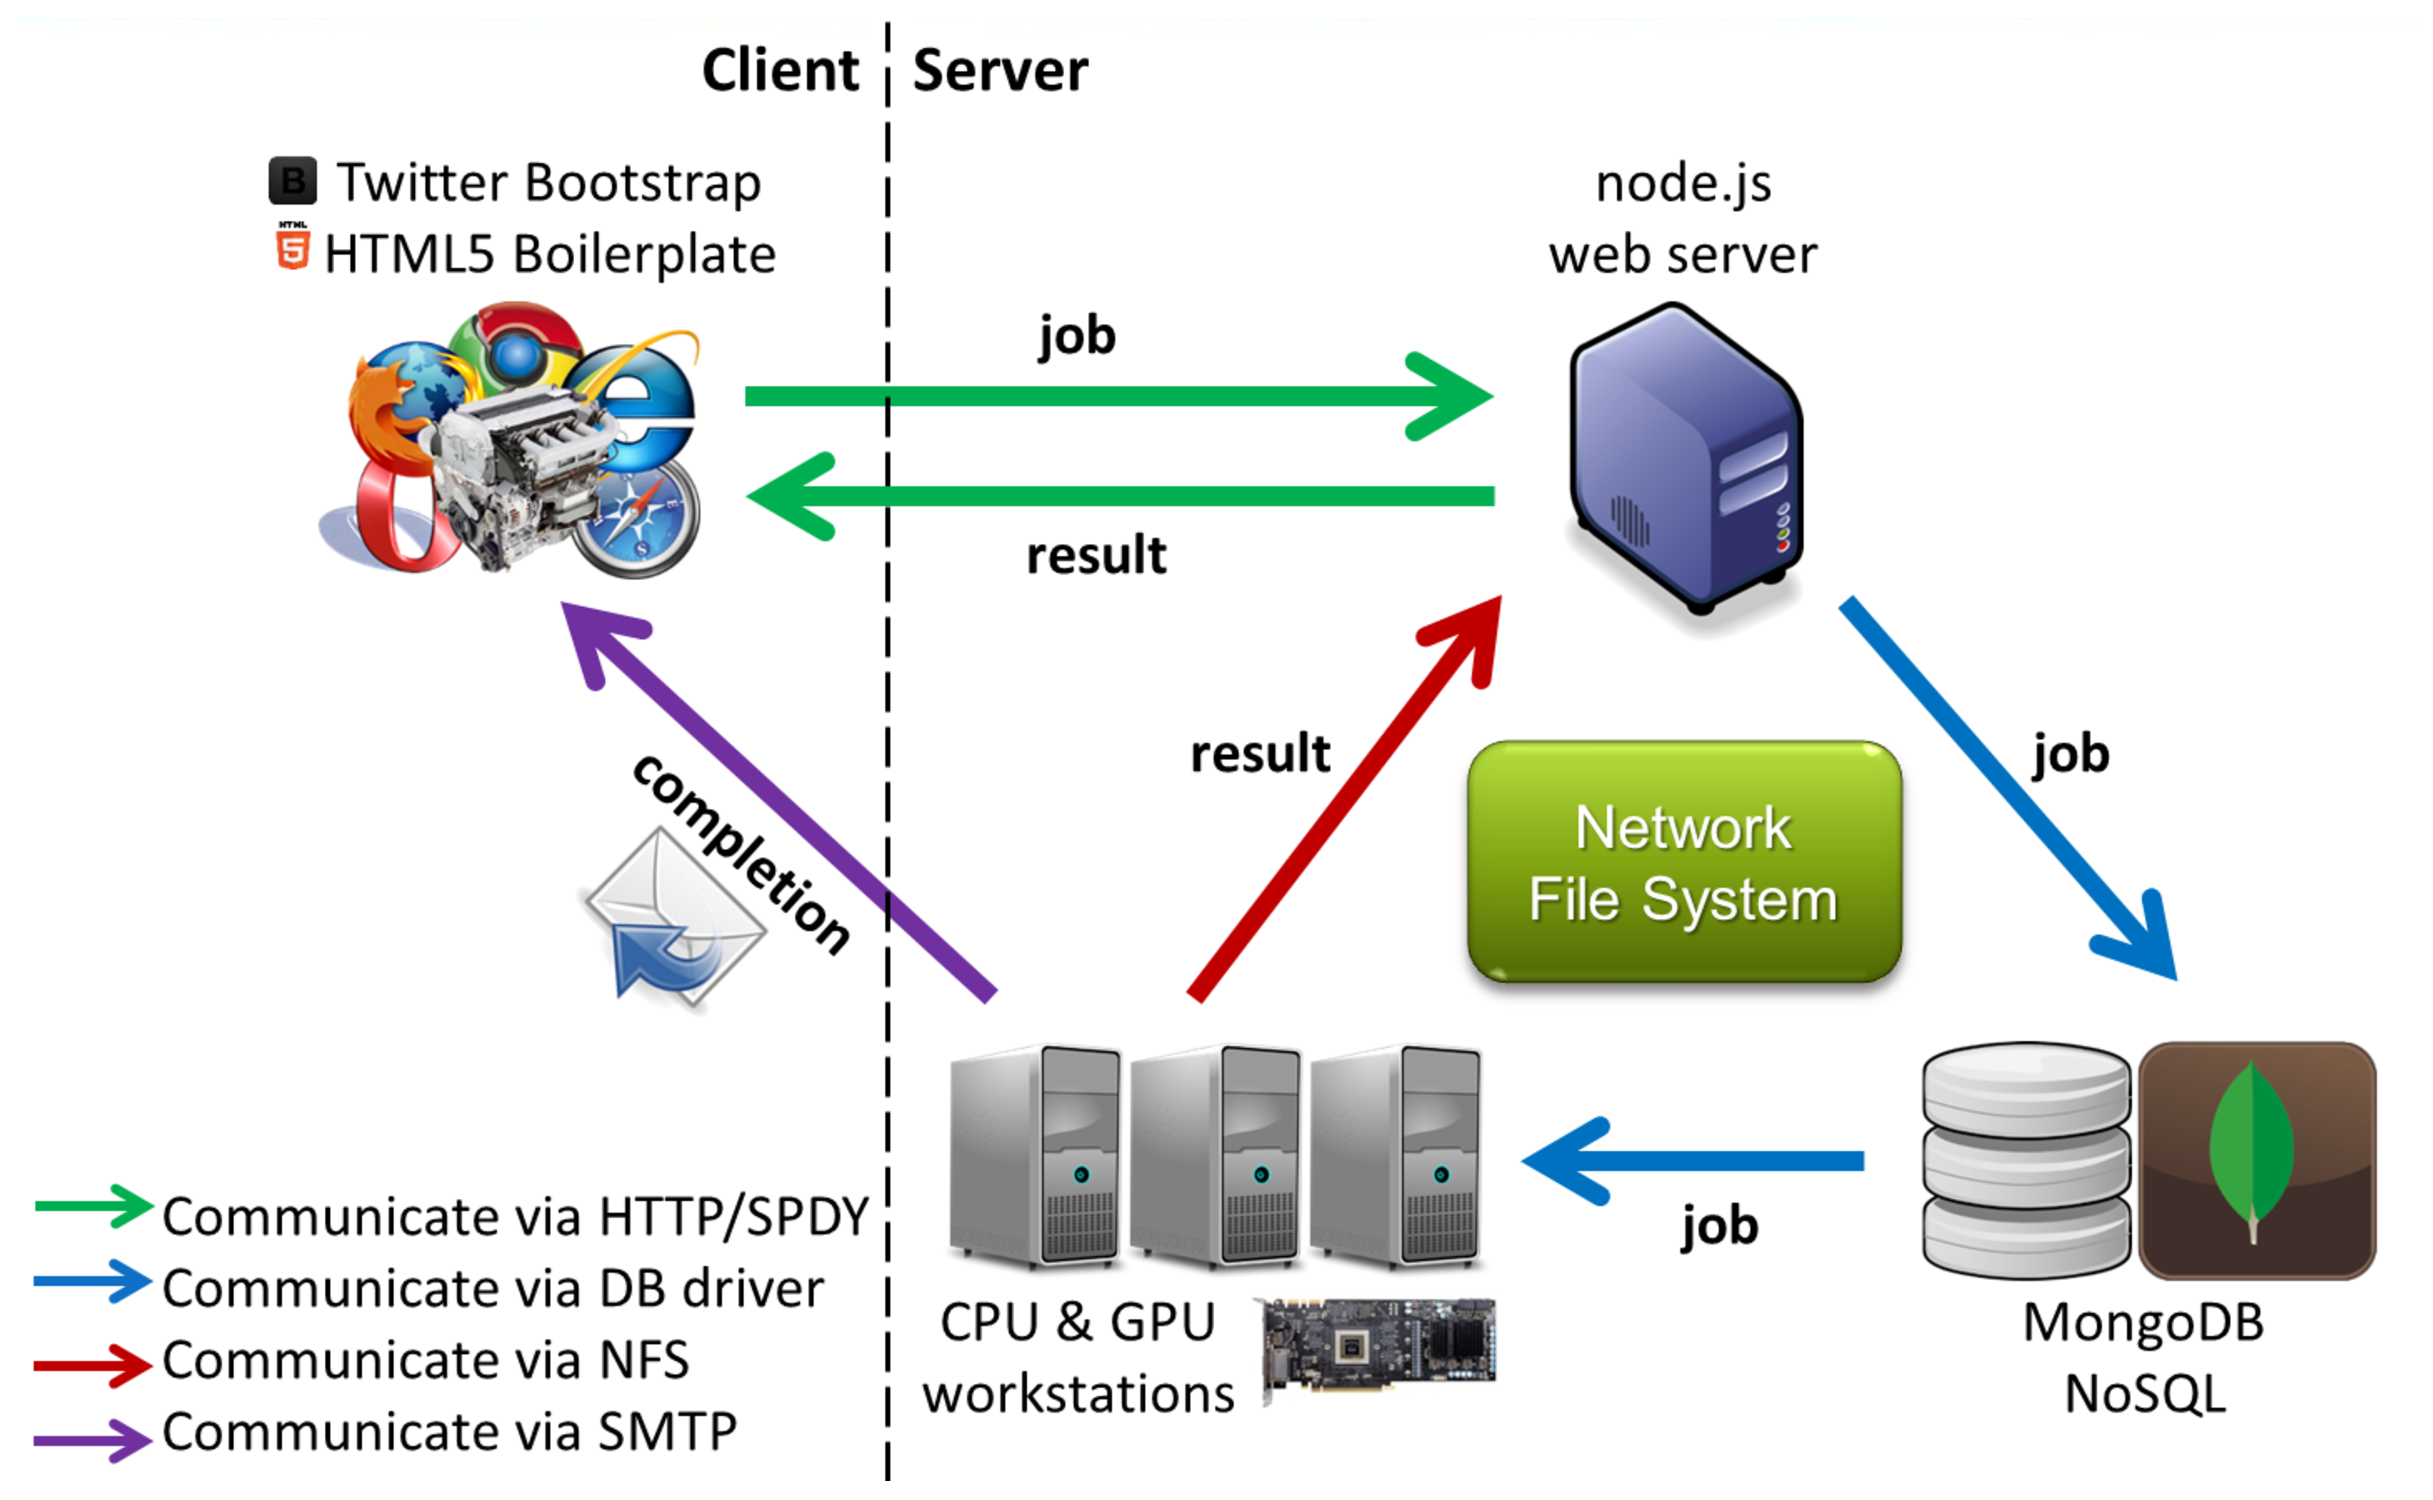
\includegraphics[width=4in]{Architecture.eps}
\end{center}
\caption{
{\bf The architecture of istar.} There are five major components: a web site, a web server, a database management system, several workstations, and a network file system.
}
\label{Architecture}
\end{figure}

\begin{figure}[!ht]
\begin{center}
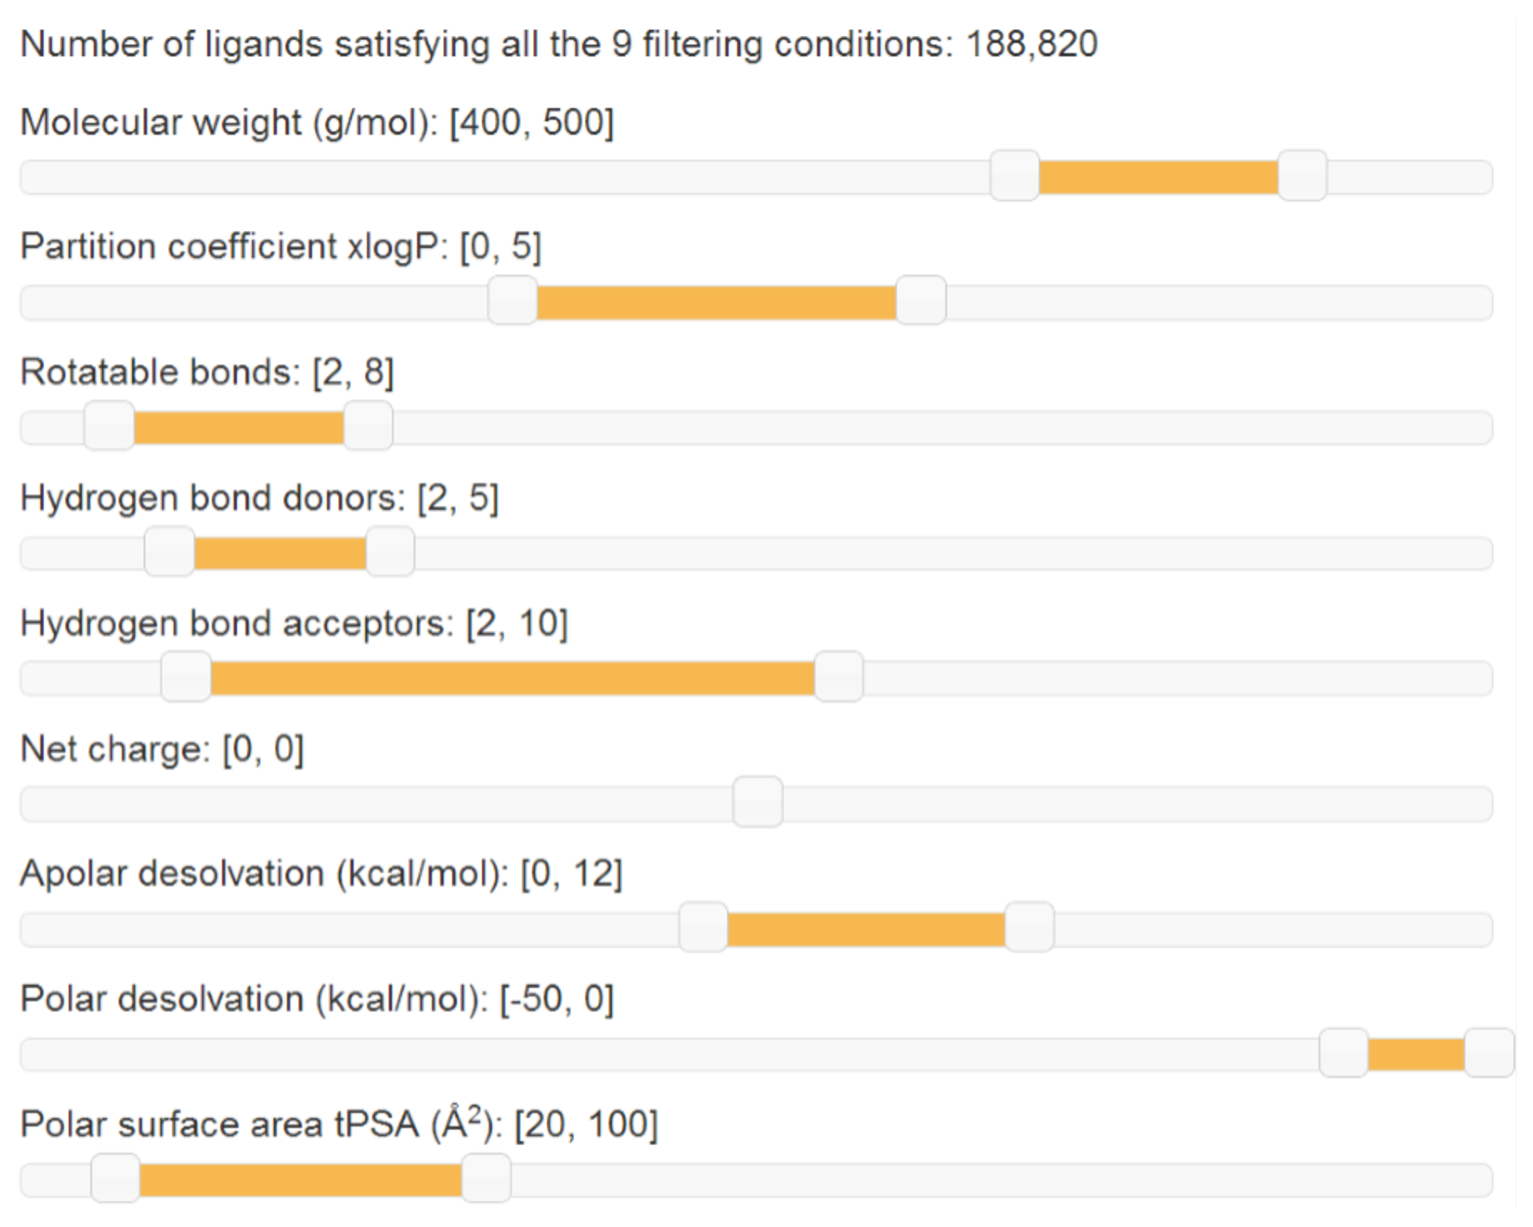
\includegraphics[width=4in]{Slider.eps}
\end{center}
\caption{
{\bf istar supports filtering ligands with molecular properties in a fine-grained manner and previewing the number of ligands to dock in real time.} Users can move the nine sliders to filter ligands in the form of closed intervals.
}
\label{Slider}
\end{figure}

\begin{figure}[!ht]
\begin{center}
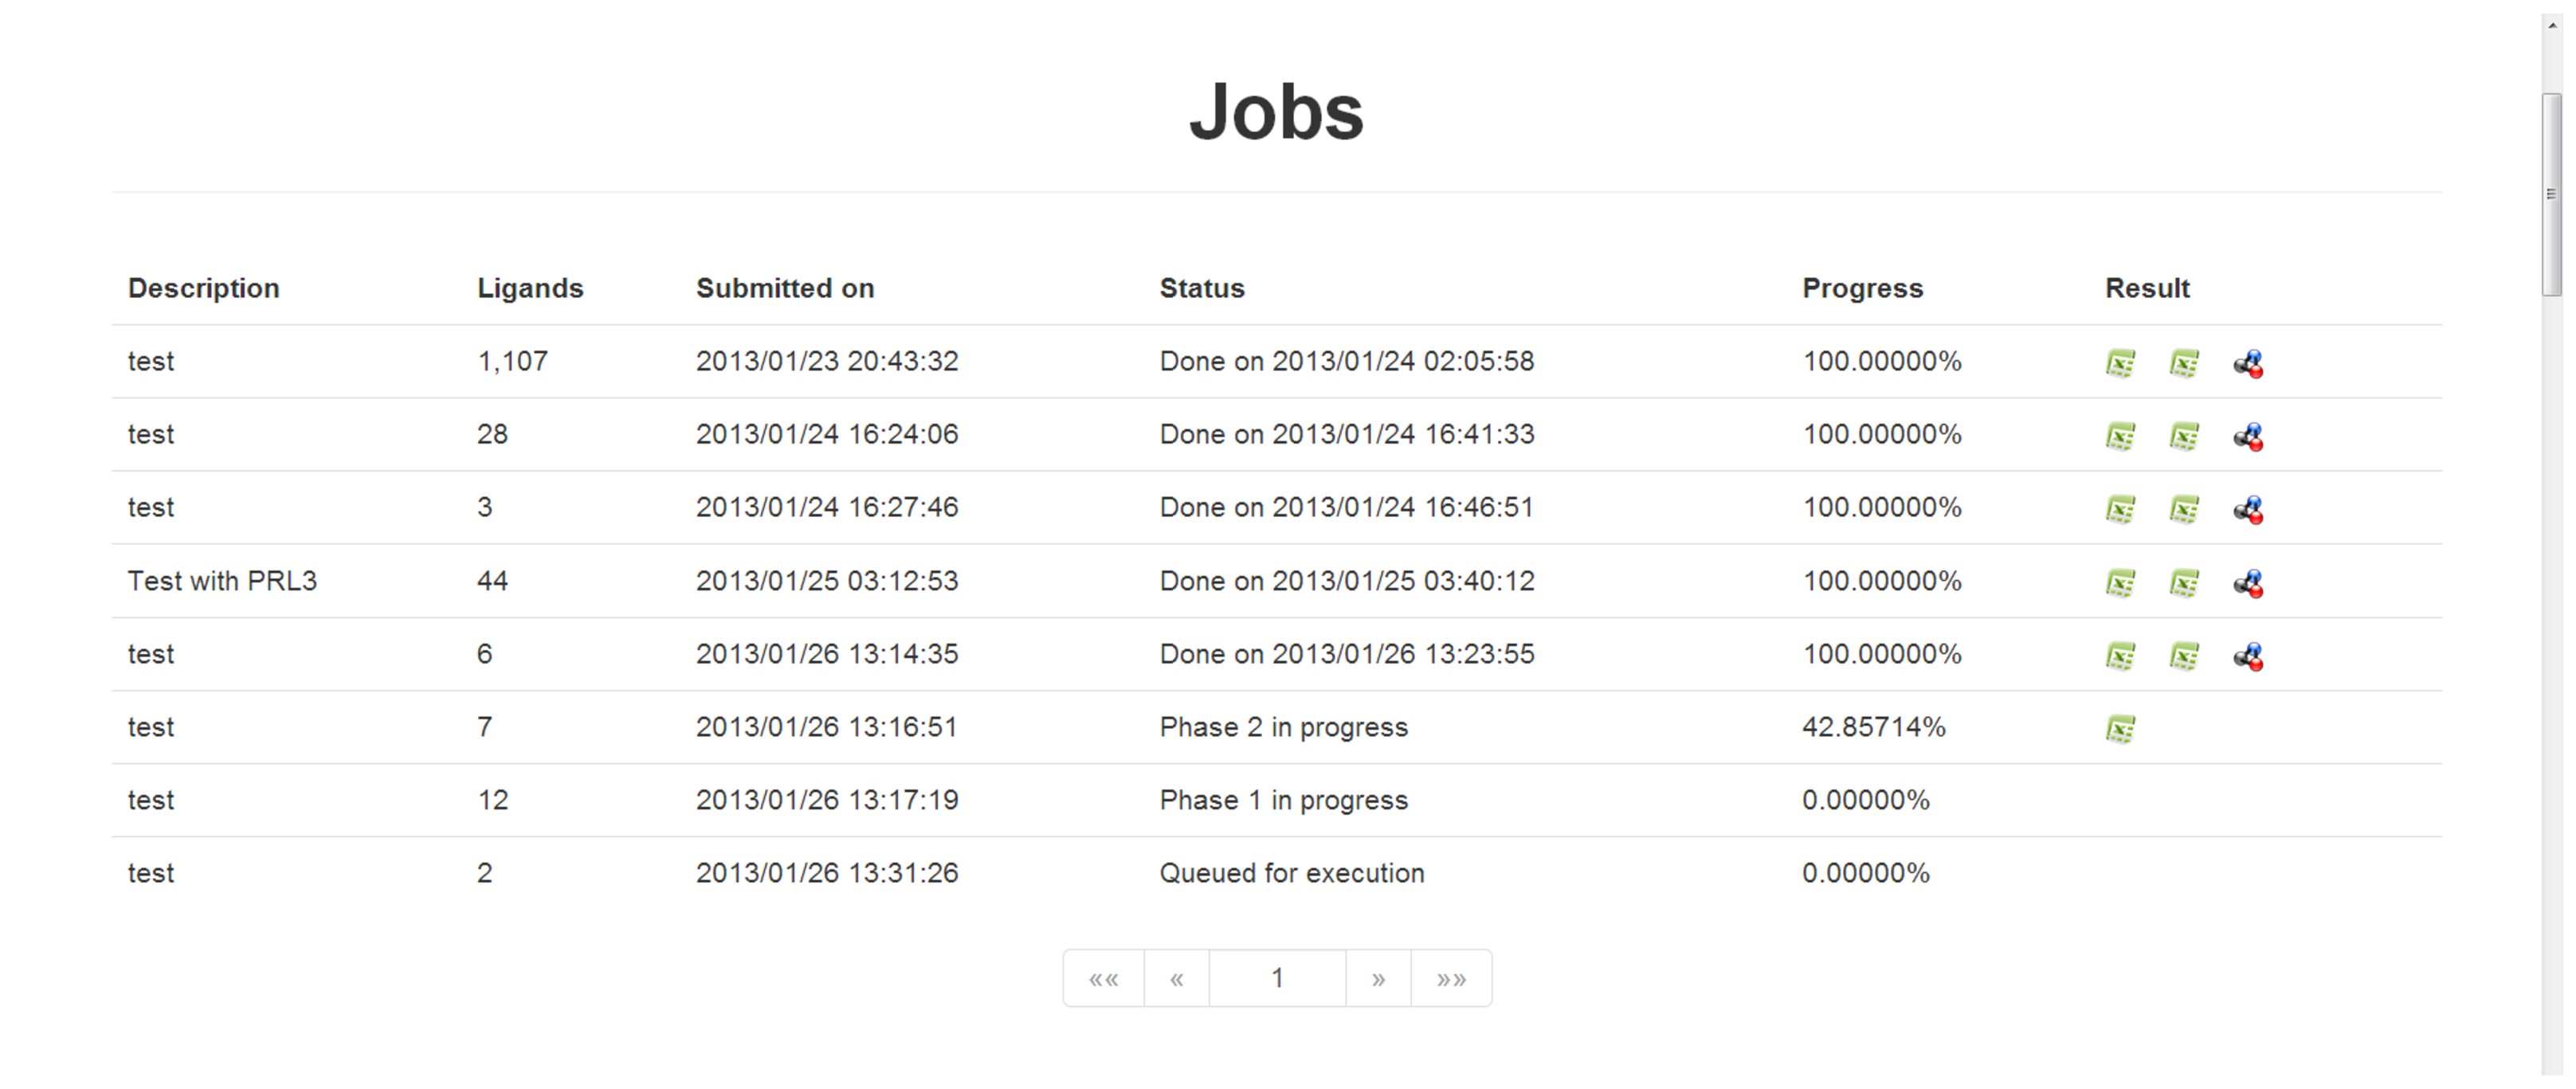
\includegraphics[width=4in]{Progress.eps}
\end{center}
\caption{
{\bf istar supports monitoring job progress in real time.} Users can thus have a rough estimation in advance of how long the jobs will take and when the jobs will complete.
}
\label{Progress}
\end{figure}

\begin{figure}[!ht]
\begin{center}
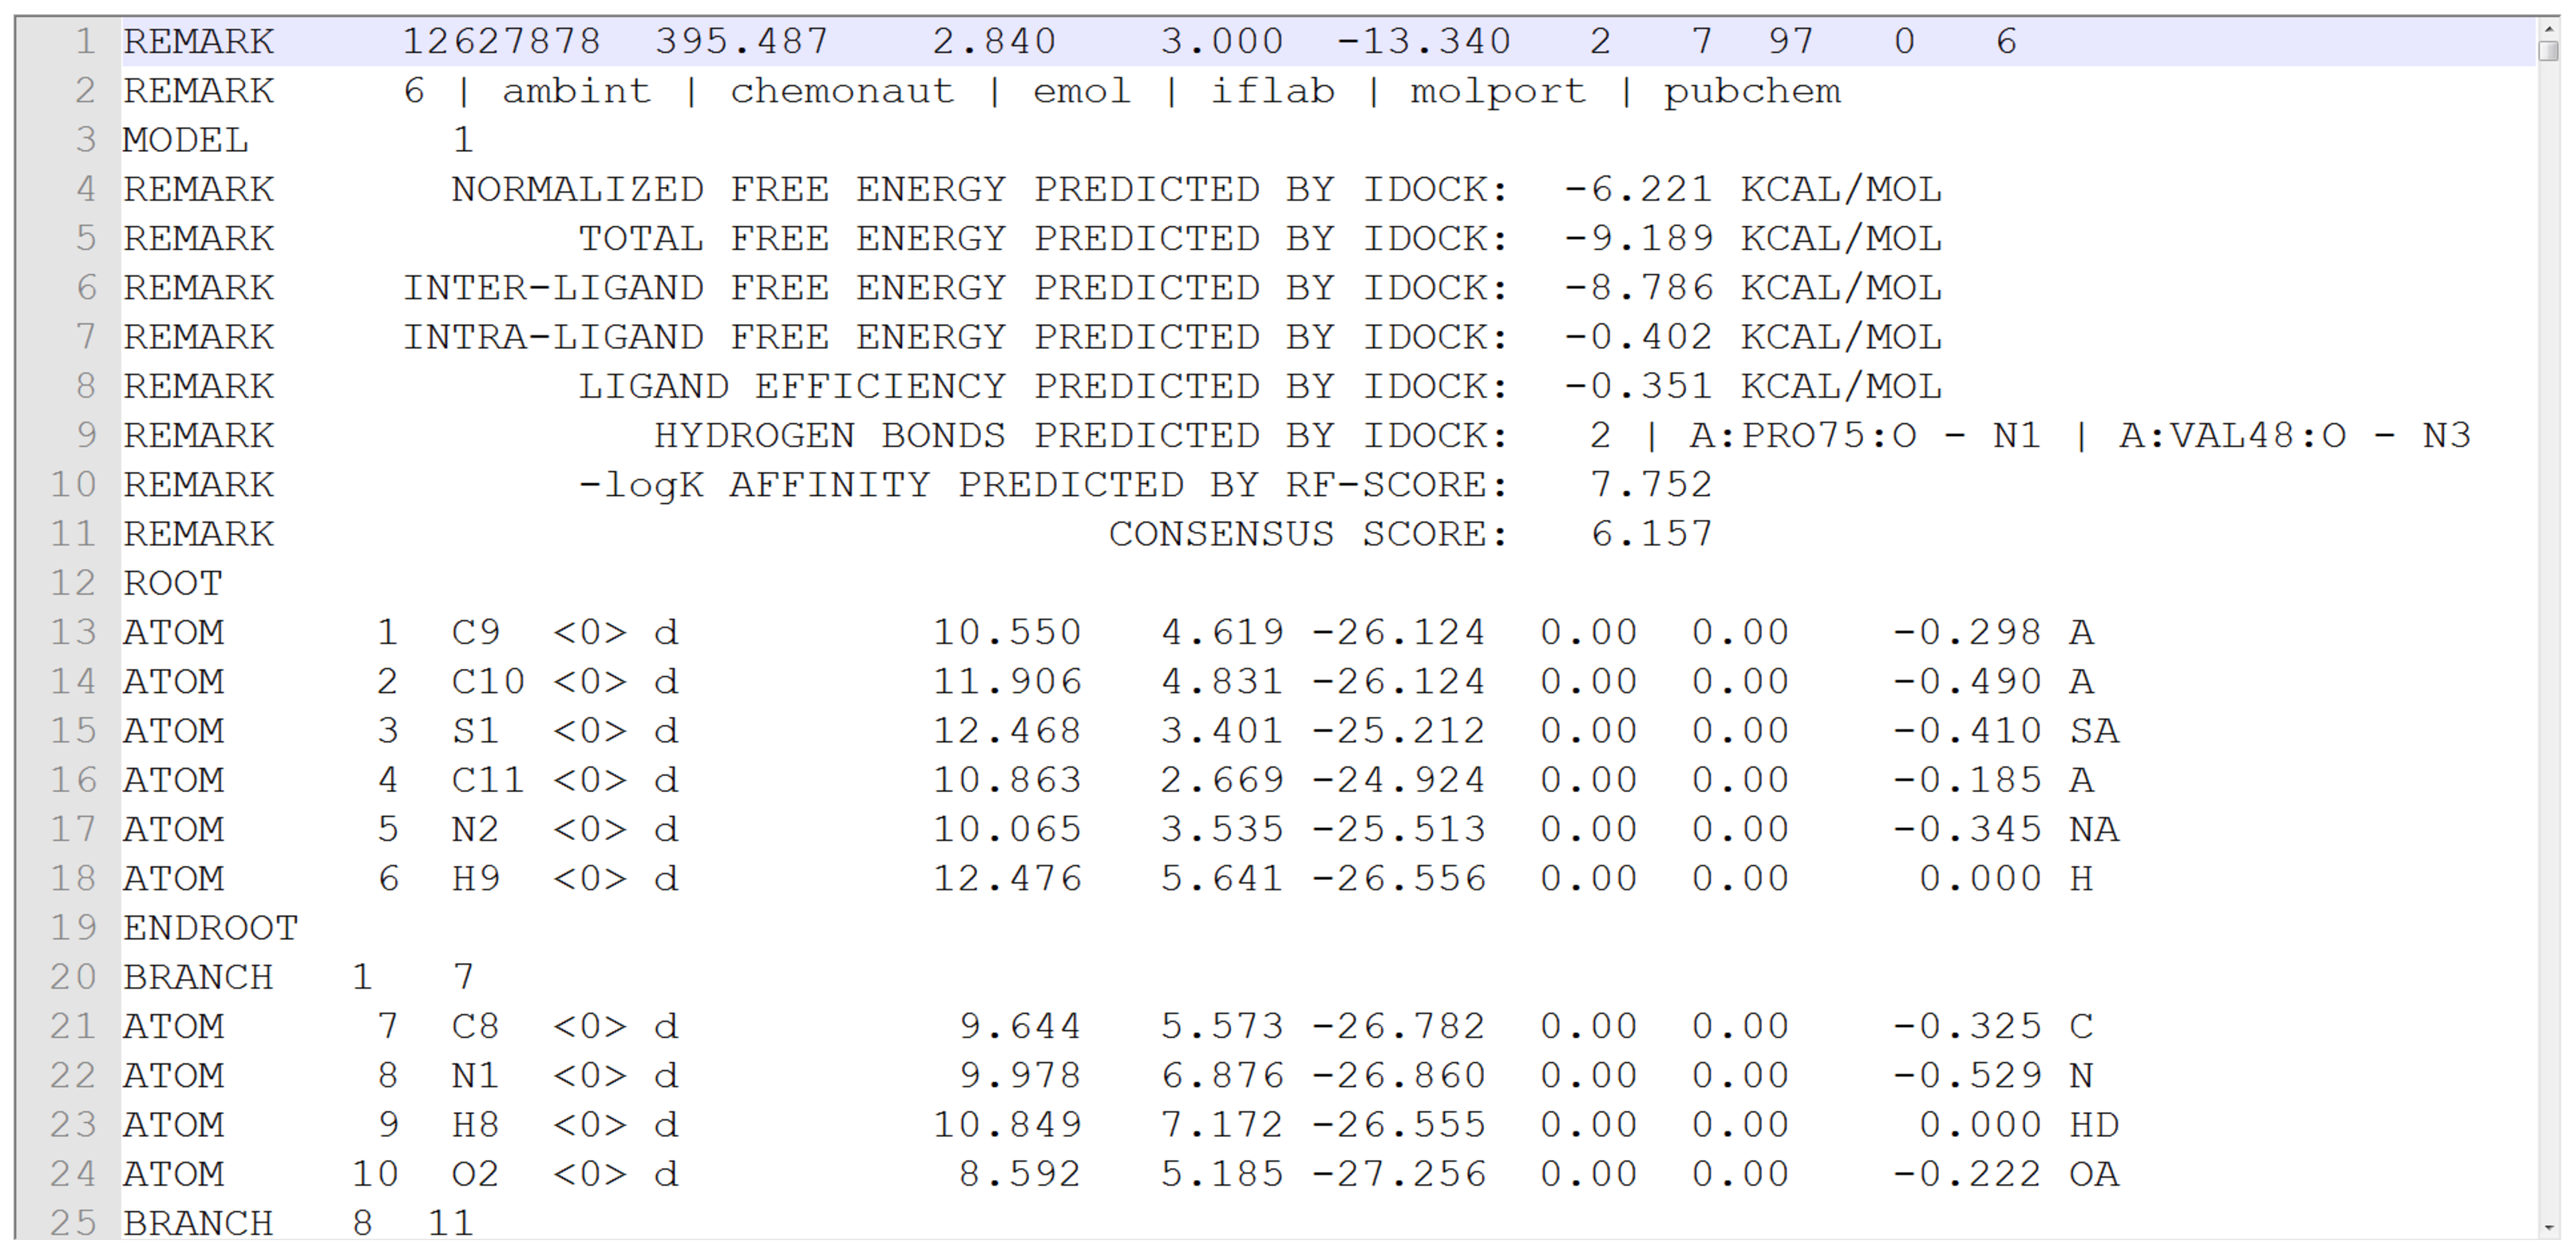
\includegraphics[width=4in]{OutputPDBQT.eps}
\end{center}
\caption{
{\bf istar writes verbose output to file in PDBQT format.} The REMARK lines describe the ZINC ID, molecular properties and suppliers of a ligand. For each predicted conformation, the REMARK lines also describe the free energy and ligand efficiency predicted by idock, putative hydrogen bonds, binding affinity predicted by RF-Score, and consensus score in pKd or pKi unit. Columns 71 to 76 of the ATOM lines describe per-atom free energy predicted by idock.
}
\label{OutputPDBQT}
\end{figure}

\begin{figure}[!ht]
\begin{center}
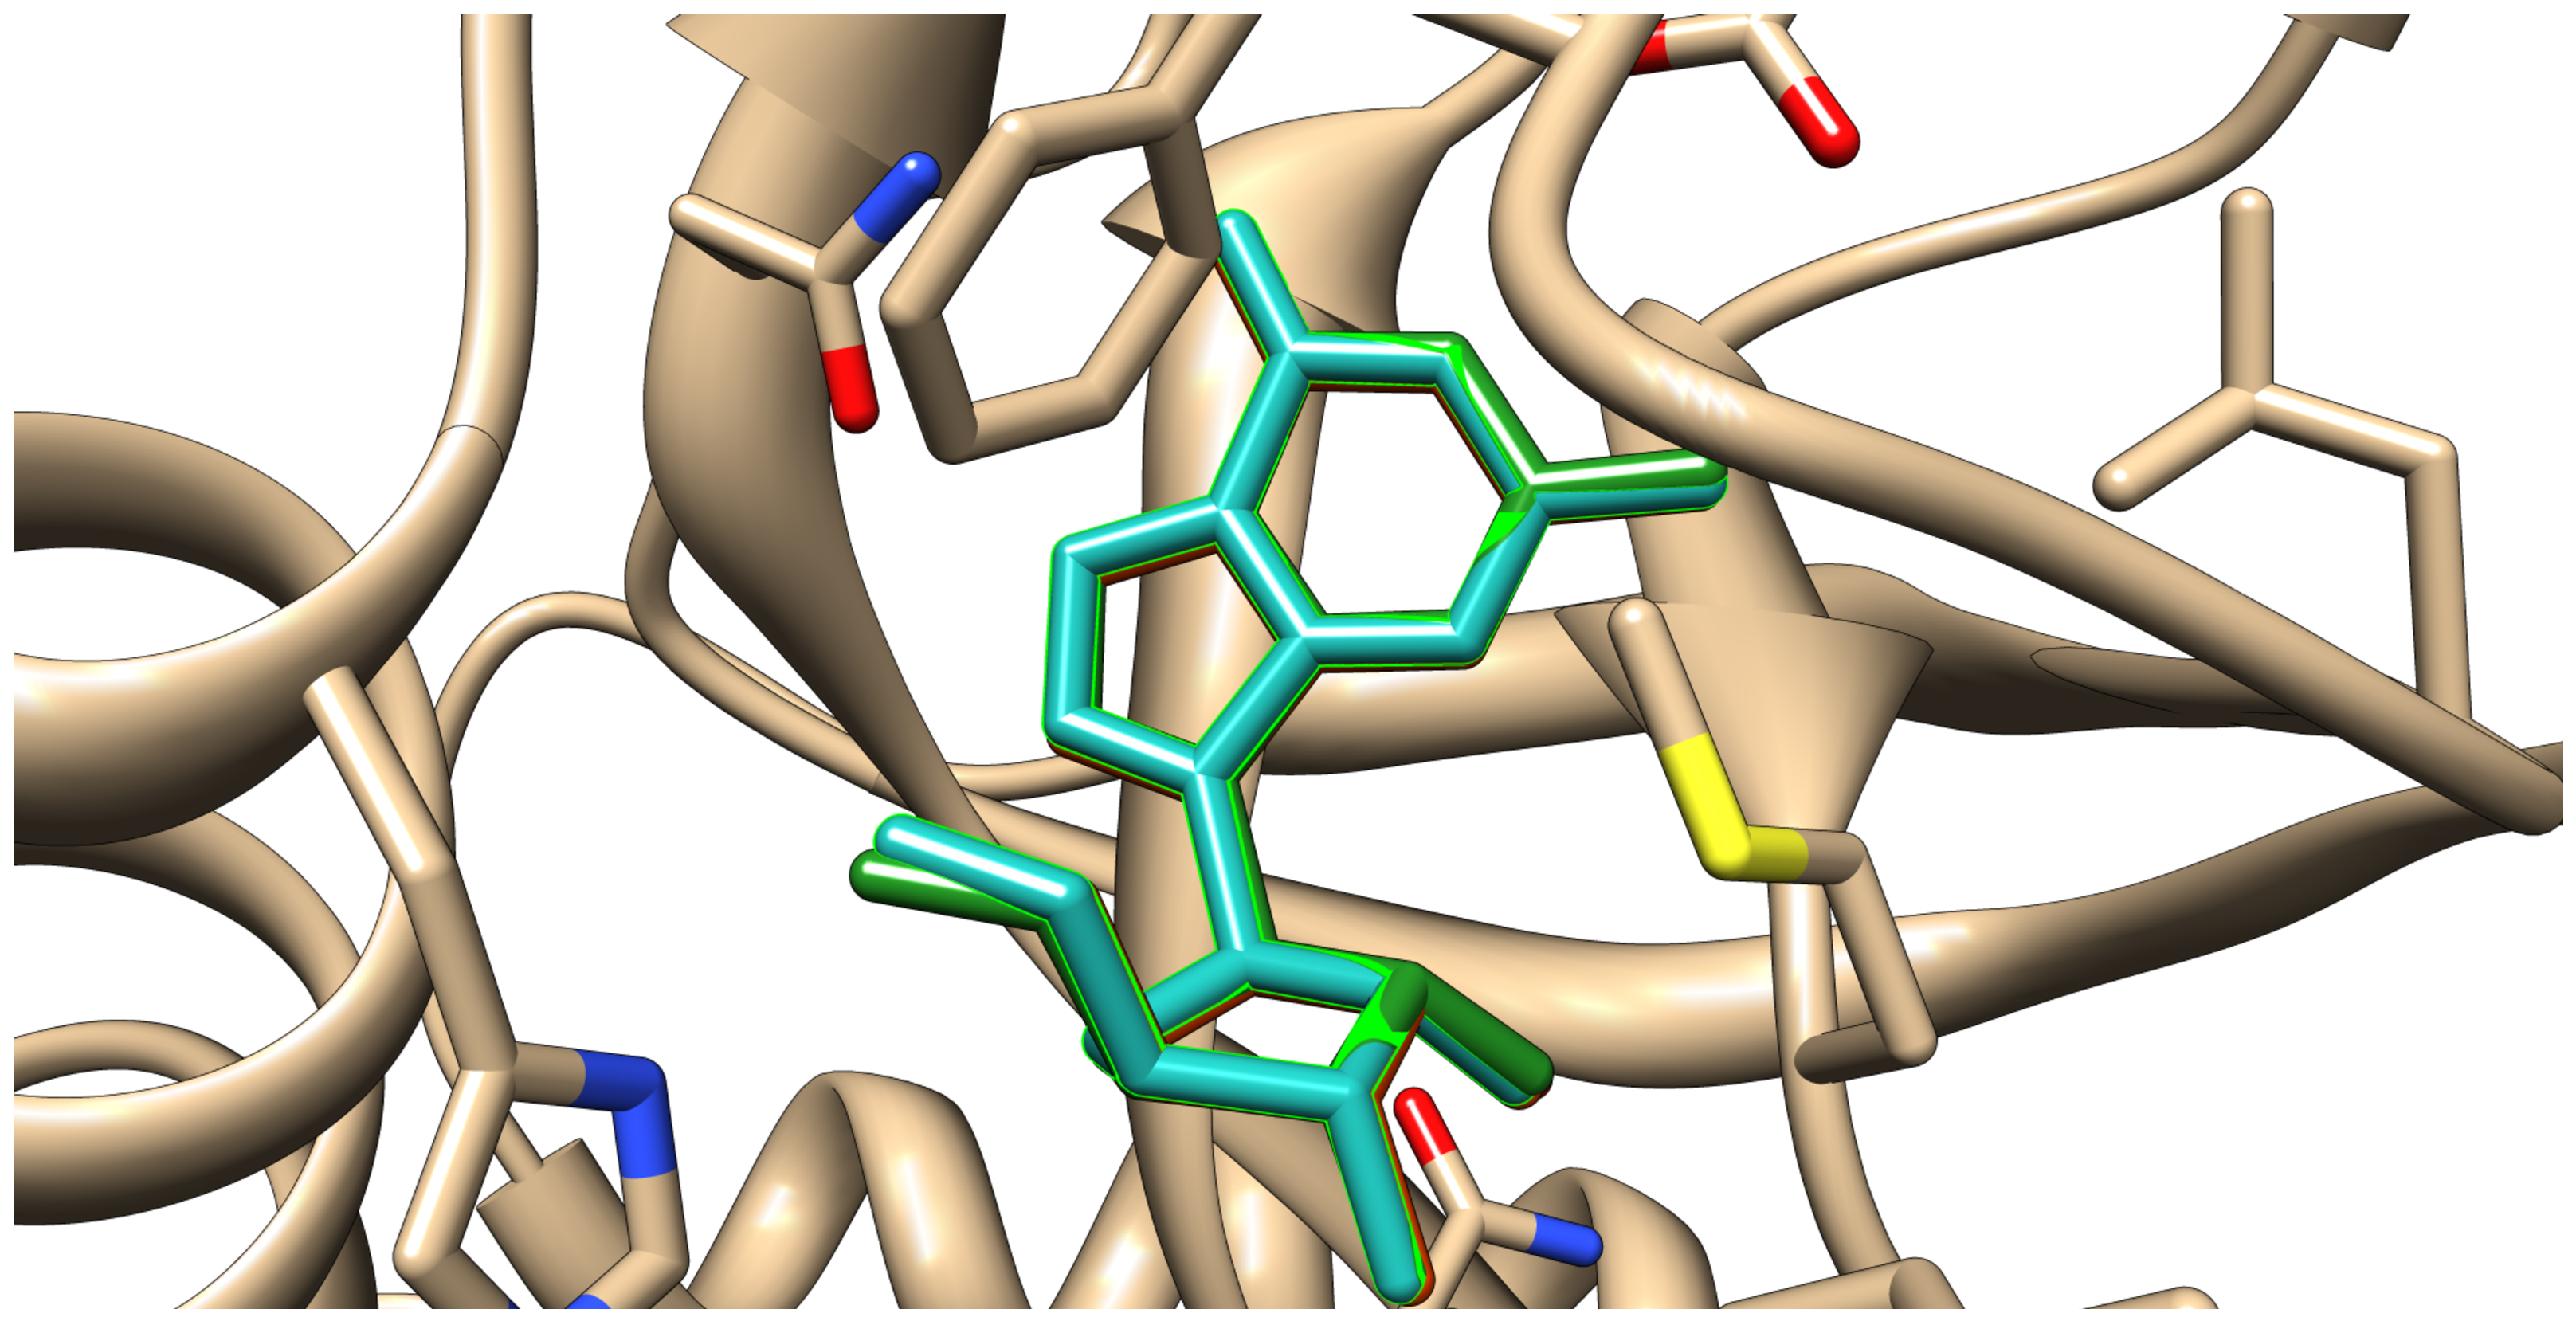
\includegraphics[width=4in]{Redocking1B8N.eps}
\end{center}
\caption{
{\bf Redocking case of PDB ID 1B8N.} The crystal conformation is rendered in green. The conformation predicted by Vina is rendered in red. The conformation predicted by idock is rendered in blue. The same color scheme applies to the subsequent three redocking cases. RMSD = 0.139\AA\ for Vina. RMSD = 0.127\AA\ for idock.
}
\label{Redocking1B8N}
\end{figure}

\begin{figure}[!ht]
\begin{center}
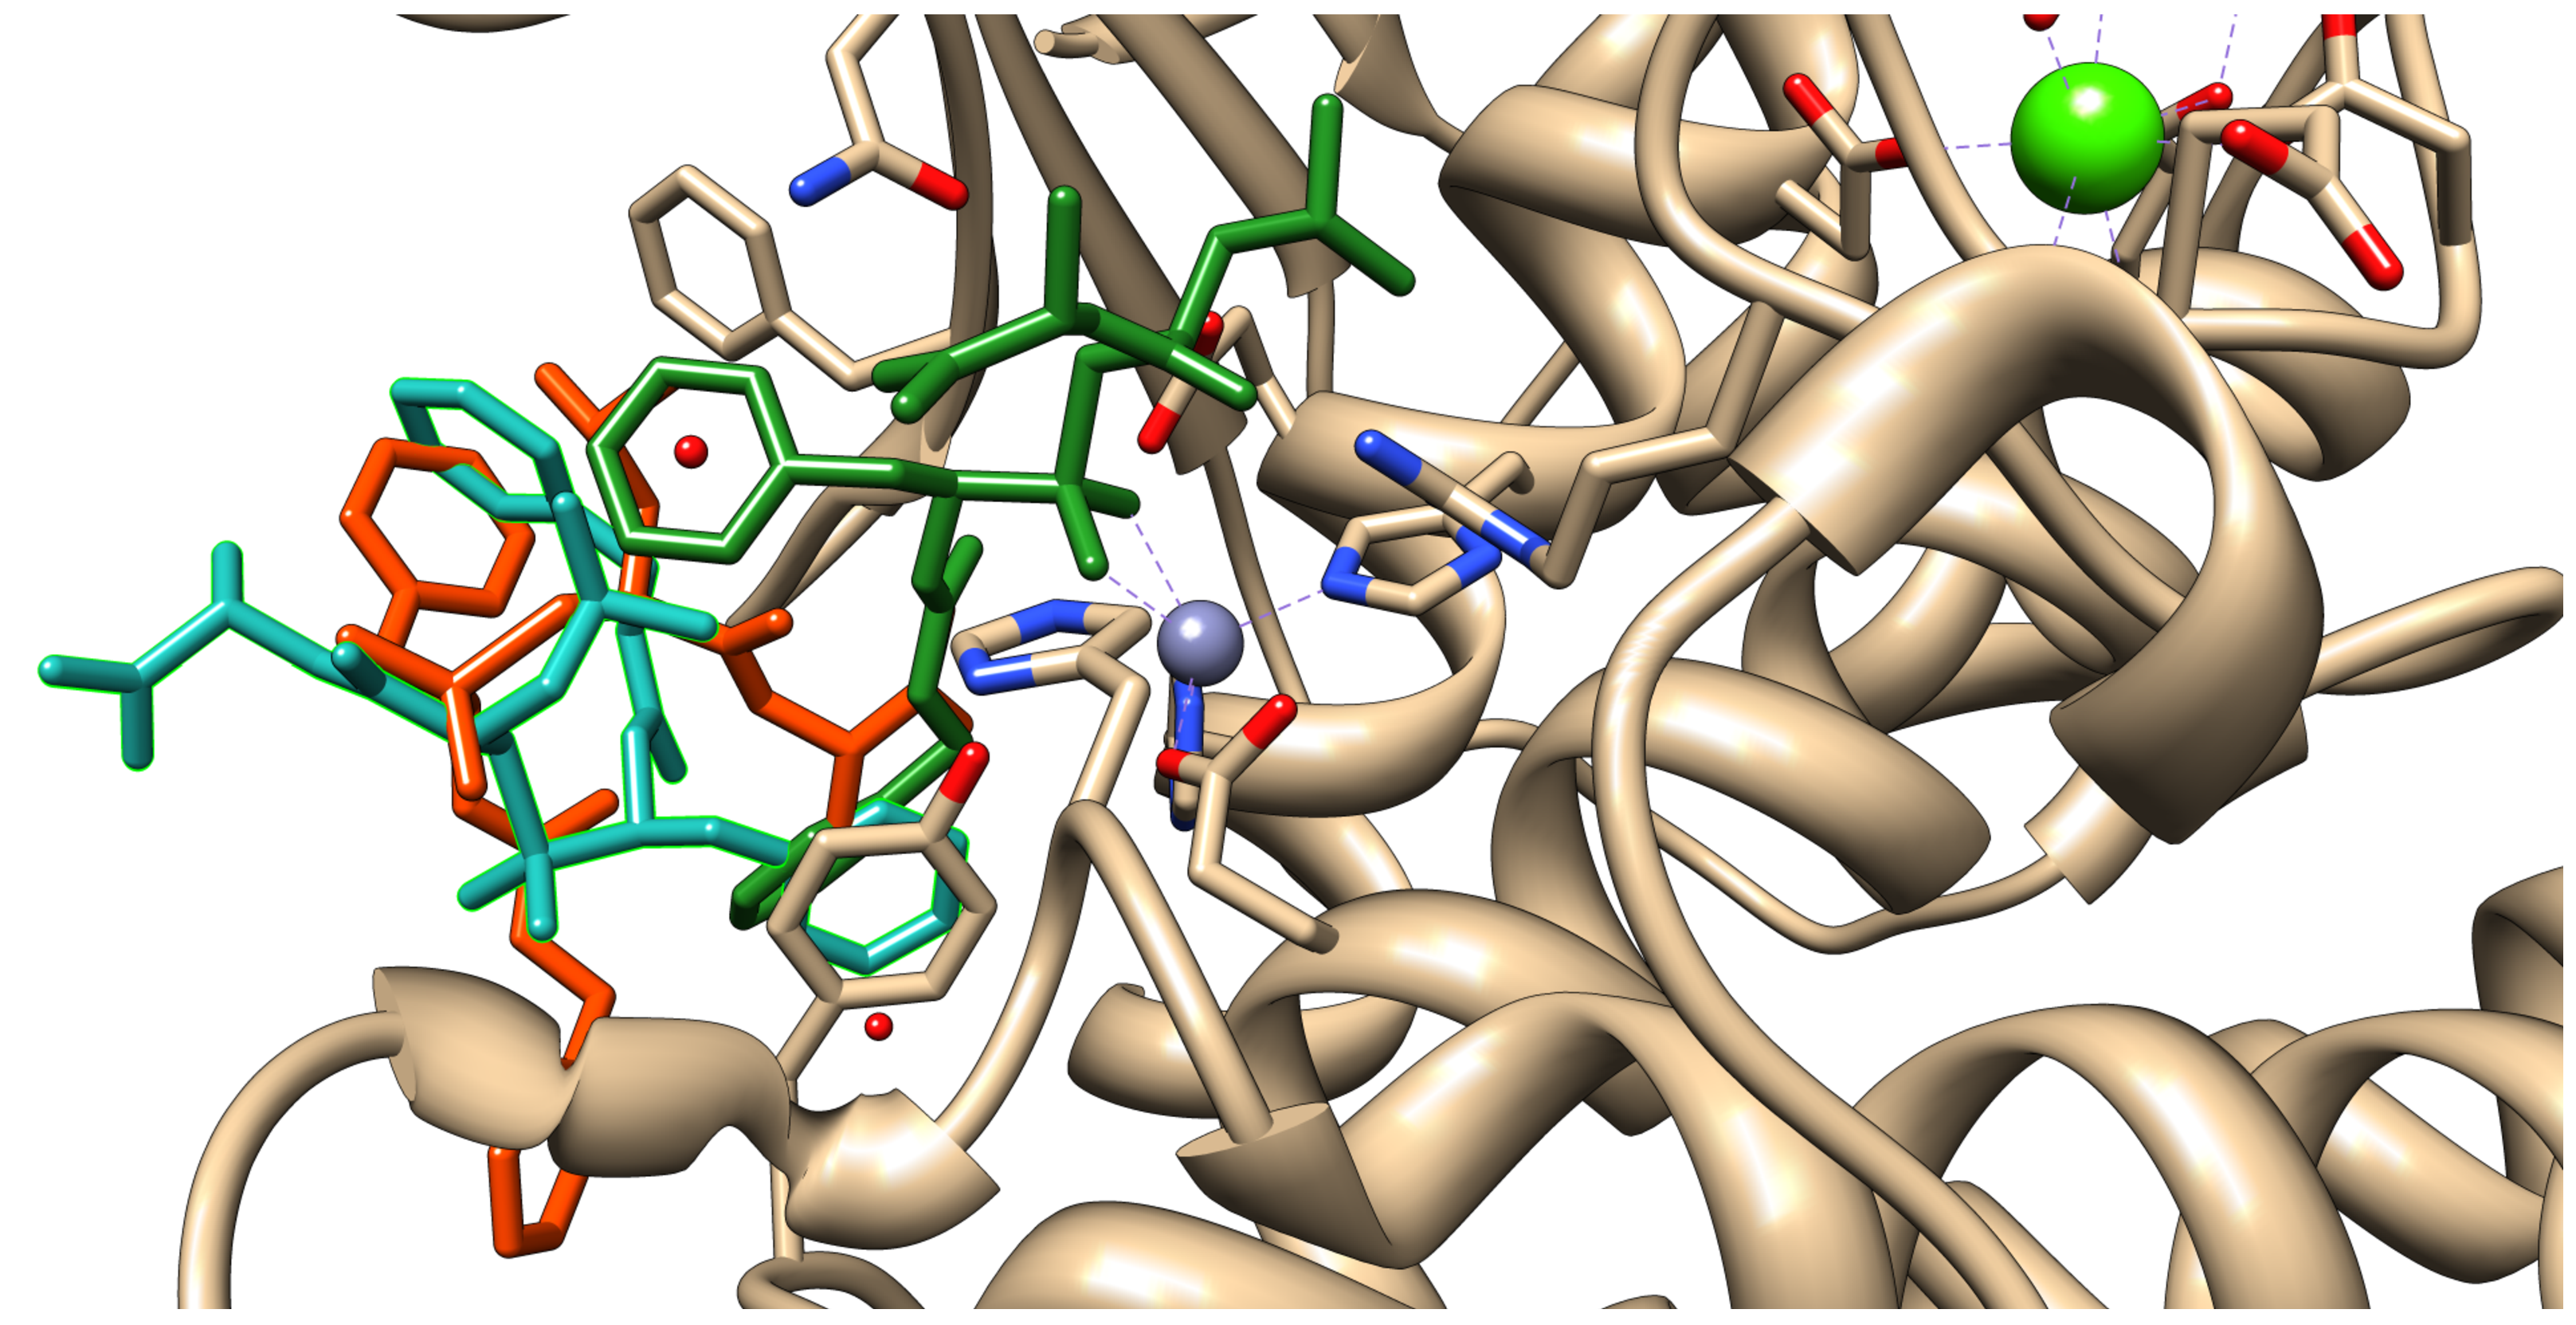
\includegraphics[width=4in]{Redocking4TMN.eps}
\end{center}
\caption{
{\bf Redocking case of PDB ID 4TMN.} RMSD = 8.401\AA\ for Vina. RMSD = 9.909\AA\ for idock.
}
\label{Redocking4TMN}
\end{figure}

\begin{figure}[!ht]
\begin{center}
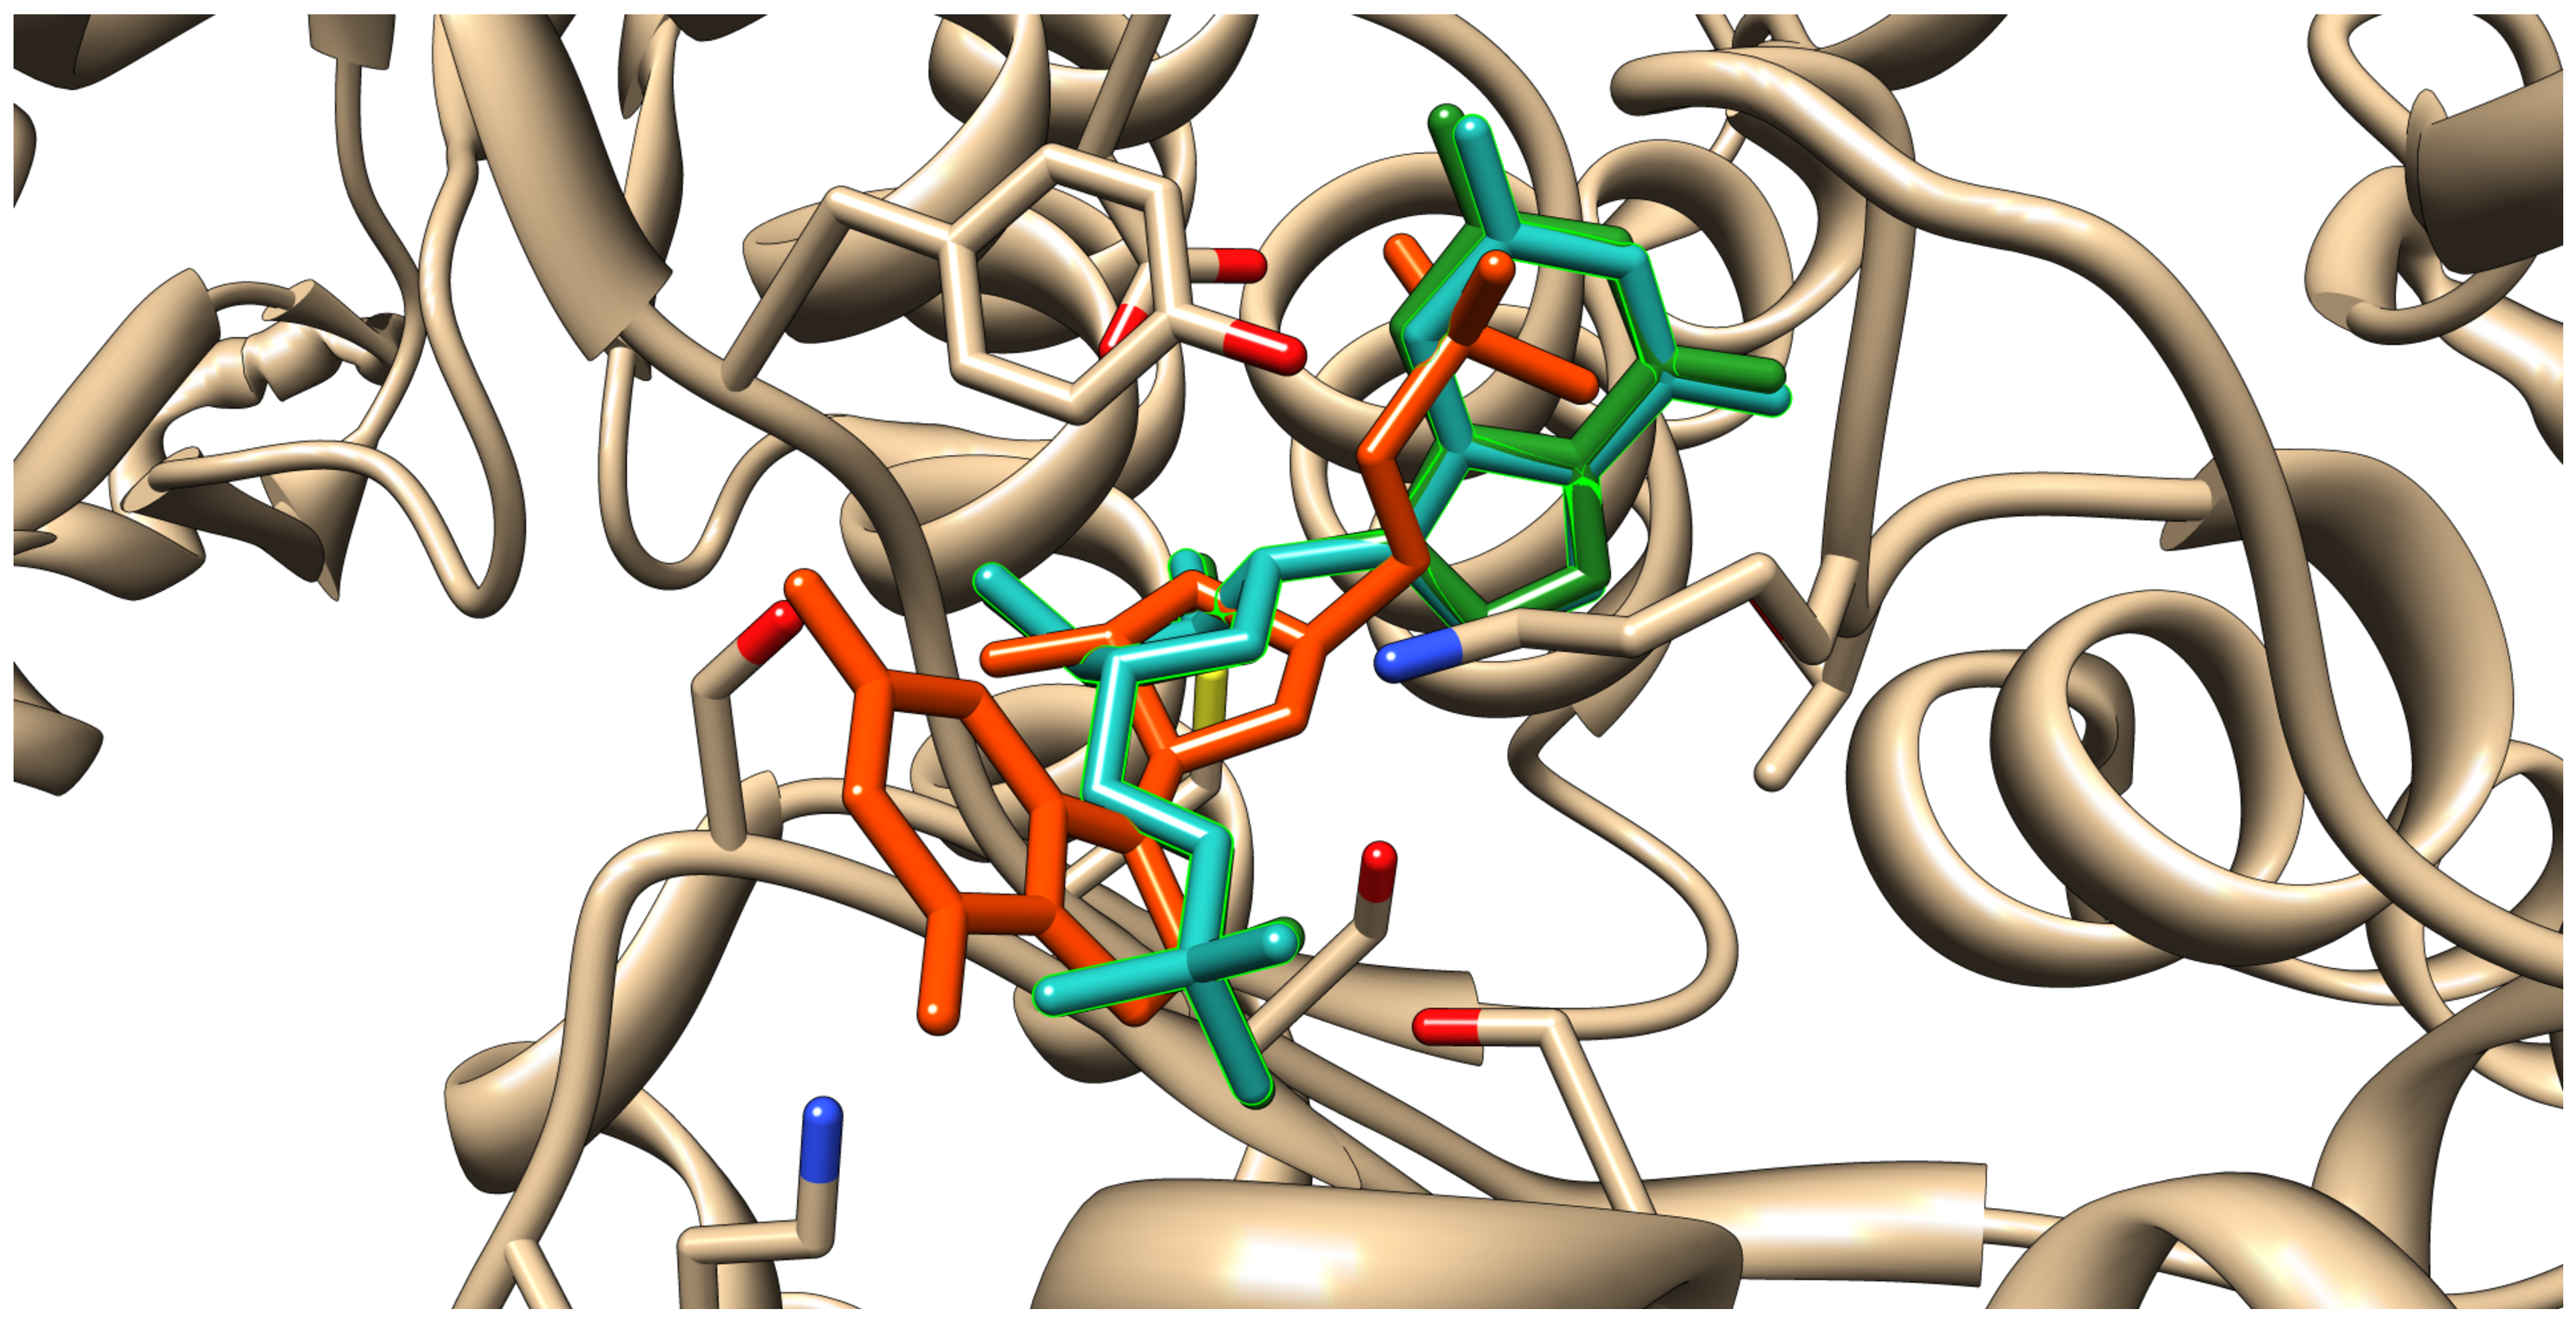
\includegraphics[width=4in]{Redocking1PKX.eps}
\end{center}
\caption{
{\bf Redocking case of PDB ID 1PKX.} RMSD = 7.059\AA\ for Vina. RMSD = 0.214\AA\ for idock.
}
\label{Redocking1PKX}
\end{figure}

\begin{figure}[!ht]
\begin{center}
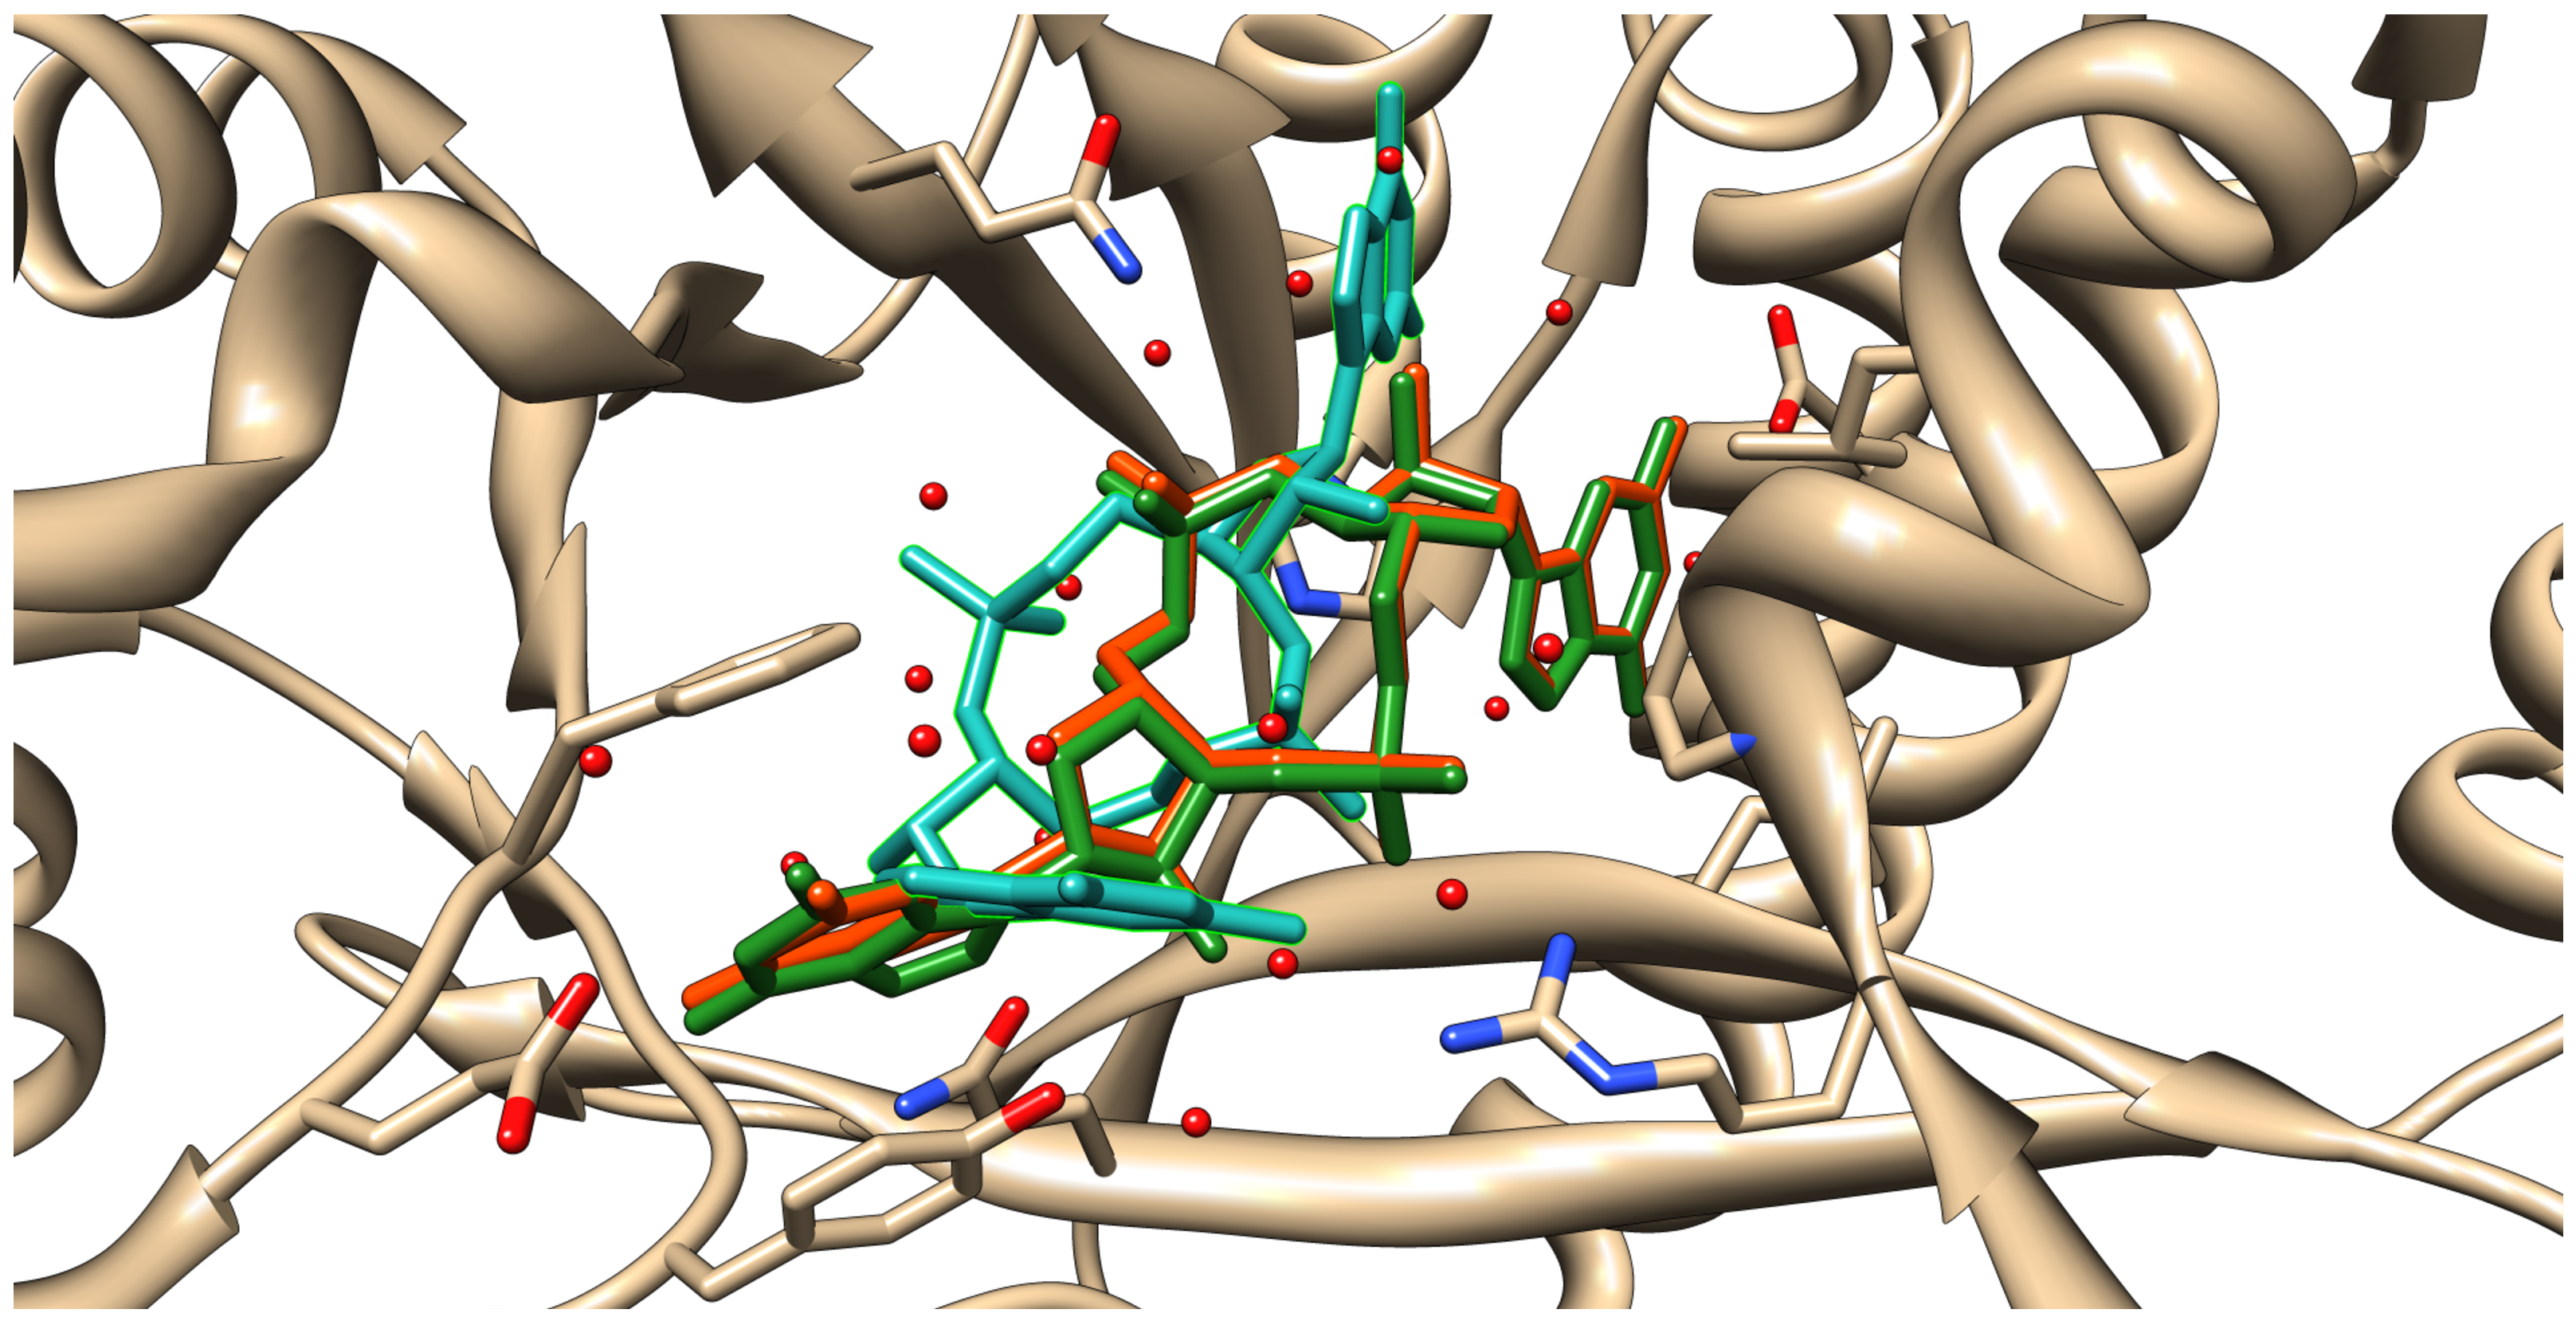
\includegraphics[width=4in]{Redocking3HV8.eps}
\end{center}
\caption{
{\bf Redocking case of PDB ID 3HV8.} RMSD = 0.290\AA\ for Vina. RMSD = 10.232\AA\ for idock.
}
\label{Redocking3HV8}
\end{figure}

\begin{figure}[!ht]
\begin{center}
\includegraphics[width=4in]{PDBbind2012Correlations.eps}
\end{center}
\caption{
{\bf Binding affinity correlation on PDBbind v2012 refined set (N = 2,897).} Along the diagonal from top left to bottom right are the distributions of experimental binding affinities and binding affinities predicted by RF-Score, AutoDock Vina, and idock, respectively. Values are in pKd or pKi unit. $R = 0.965, R_s = 0.966, RMSE = 0.60, SD = 0.60$ for RF-Score, $R = 0.466, R_s = 0.464, RMSE = 2.29, SD = 2.21$ for Vina, $R = 0.451, R_s = 0.453, RMSE = 2.28, SD = 2.25$ for idock.
}
\label{PDBbind2012Correlations}
\end{figure}

\begin{figure}[!ht]
\begin{center}
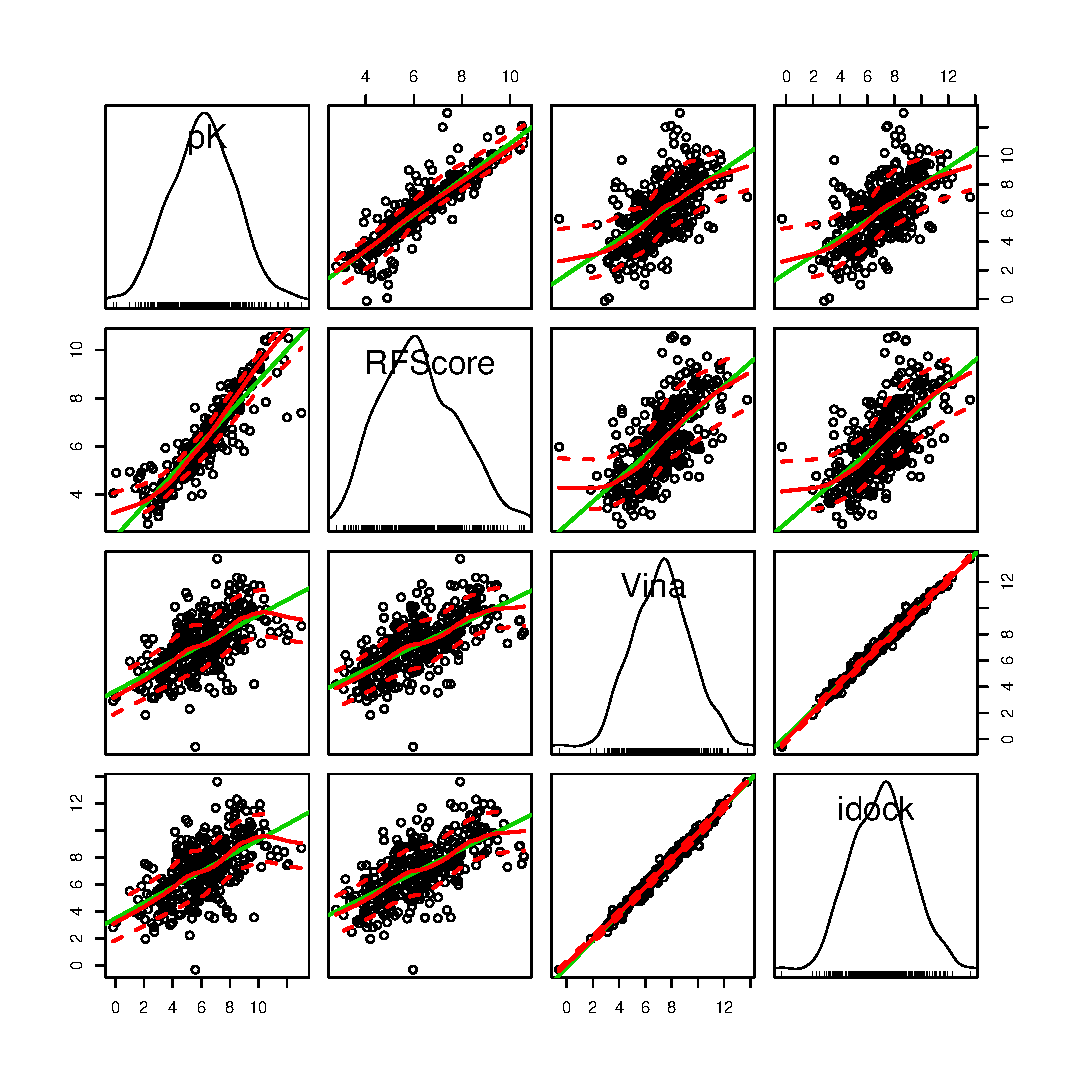
\includegraphics[width=4in]{CSAR2010Correlations.eps}
\end{center}
\caption{
{\bf Binding affinity correlation on CSAR NRC HiQ Set 24Sept2010 (N = 343).} Along the diagonal from top left to bottom right are the distributions of experimental binding affinities and binding affinities predicted by RF-Score, AutoDock Vina, and idock, respectively. Values are in pKd or pKi unit. $R = 0.899, R_s = 0.926, RMSE = 1.05, SD = 1.05$ for RF-Score, $R = 0.595, R_s = 0.611, RMSE = 2.26, SD = 1.98$ for Vina, $R = 0.597, R_s = 0.613, RMSE = 2.17, SD = 1.97$ for idock.
}
\label{CSAR2010Correlations}
\end{figure}

\begin{figure}[!ht]
\begin{center}
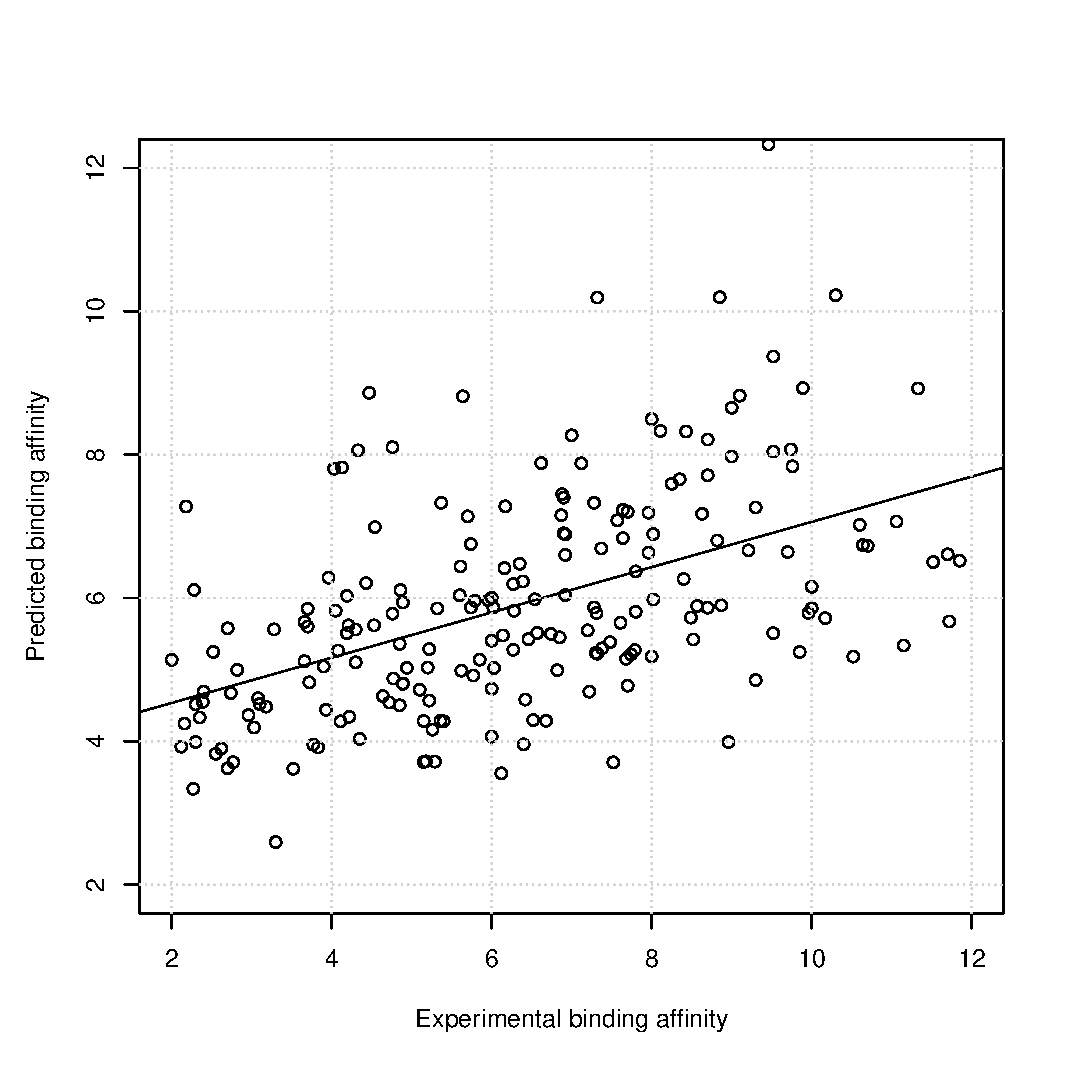
\includegraphics[width=4in]{pK-idockConf1idock.eps}
\end{center}
\caption{
{\bf Scatter plot of predicted binding affinity of docked pose against experimental binding affinity on PDBbind v2012 core set (N = 201).} $R = 0.502, R_s = 0.530, RMSE = 2.15, SD = 2.11$
}
\label{pK-idockConf1idock}
\end{figure}

\begin{figure}[!ht]
\begin{center}
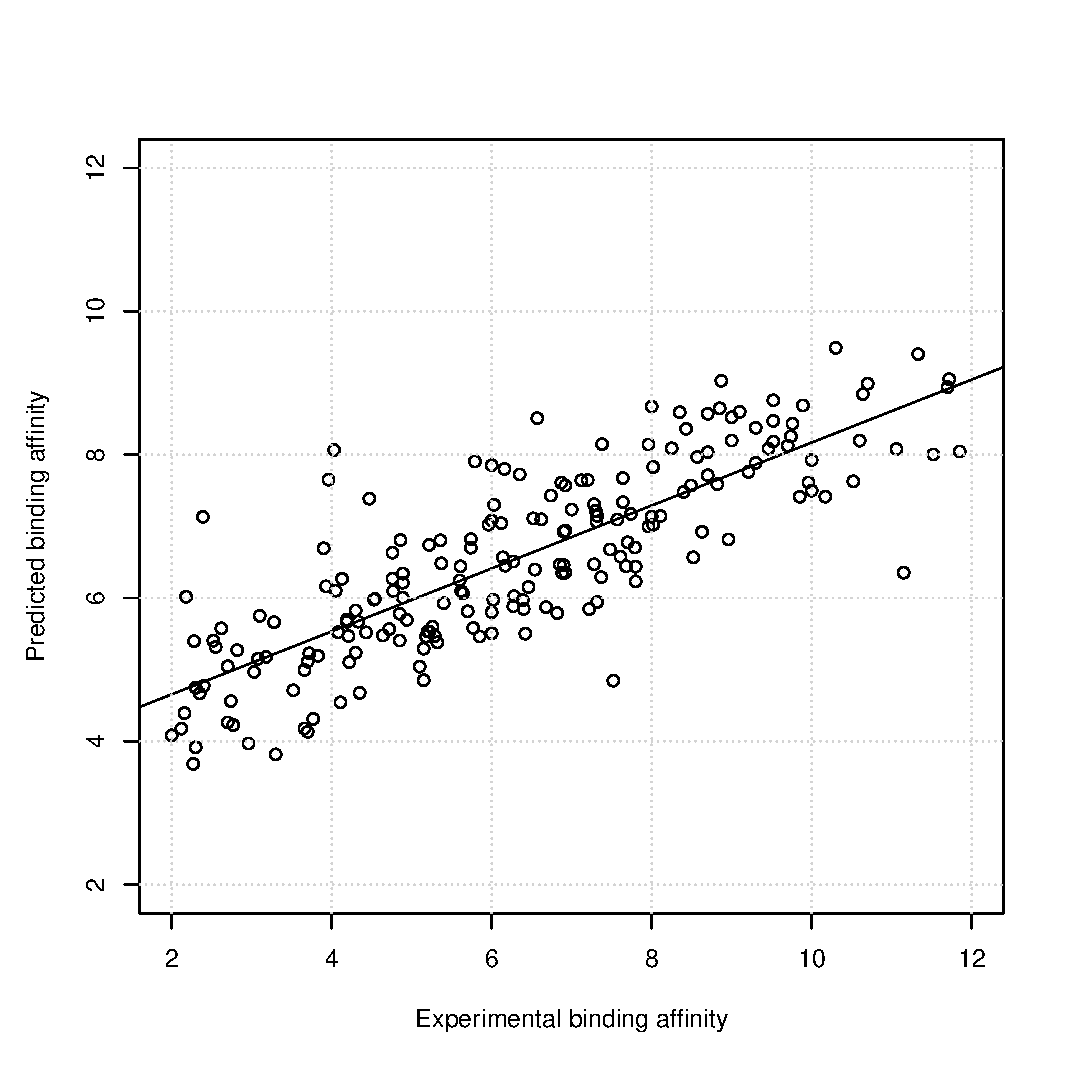
\includegraphics[width=4in]{pK-idockConfsRFScoreMax.eps}
\end{center}
\caption{
{\bf Scatter plot of predicted binding affinity of docked pose against experimental binding affinity on PDBbind v2012 core set (N = 201).} $R = 0.815, R_s = 0.817, RMSE = 1.57, SD = 1.55$
}
\label{pK-idockConfsRFScoreMax}
\end{figure}

\begin{figure}[!ht]
\begin{center}
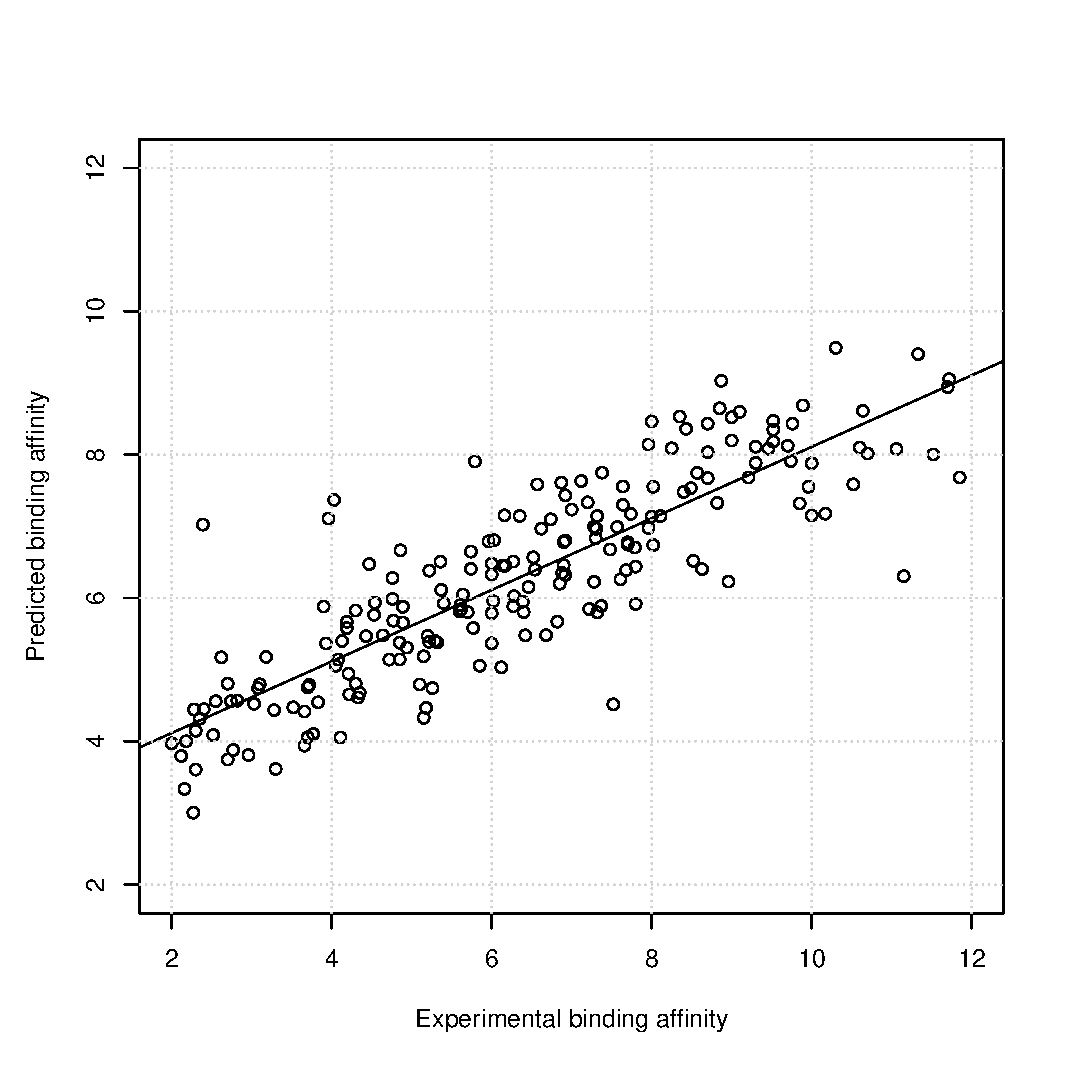
\includegraphics[width=4in]{pK-idockConf1RFScore.eps}
\end{center}
\caption{
{\bf Scatter plot of predicted binding affinity of docked pose against experimental binding affinity on PDBbind v2012 core set (N = 201).} $R = 0.855, R_s = 0.859, RMSE = 1.41, SD = 1.42$
}
\label{pK-idockConf1RFScore}
\end{figure}

\section*{Tables}

\begin{table}[!ht]
\caption{
\bf{Redocking success rates}}
\begin{tabular}{lrrrrrr}
\hline
& \multicolumn{2}{c}{PDBbind v2012} & \multicolumn{2}{c}{PDBbind v2011} & \multicolumn{2}{c}{CSAR NRC HiQ}\\
Condition & idock & Vina & idock & Vina & idock & Vina\\
\hline
RMSD1 = RMSDm & 49\% & 53\% & 47\% & 54\% & 57\% & 71\%\\
RMSD2 = RMSDm & 15\% & 16\% & 16\% & 14\% & 17\% & 13\%\\
RMSD3 = RMSDm &  8\% &  7\% &  8\% &  8\% &  7\% &  4\%\\
RMSD4 = RMSDm &  6\% &  6\% &  6\% &  5\% &  5\% &  3\%\\
RMSD5 = RMSDm &  5\% &  4\% &  5\% &  5\% &  4\% &  1\%\\
RMSD6 = RMSDm &  5\% &  3\% &  5\% &  4\% &  3\% &  3\%\\
RMSD7 = RMSDm &  4\% &  4\% &  5\% &  4\% &  1\% &  2\%\\
RMSD8 = RMSDm &  5\% &  3\% &  4\% &  3\% &  3\% &  2\%\\
RMSD9 = RMSDm &  4\% &  3\% &  4\% &  3\% &  3\% &  2\%\\
\noalign{\smallskip}
RMSD1 \textless\ 0.5 \AA & 10\% & 12\% & 11\% & 12\% & 21\% & 21\%\\
RMSD1 \textless\ 1.0 \AA & 26\% & 31\% & 29\% & 31\% & 40\% & 47\%\\
RMSD1 \textless\ 1.5 \AA & 43\% & 47\% & 45\% & 47\% & 61\% & 67\%\\
RMSD1 \textless\ 2.0 \AA & 51\% & 56\% & 53\% & 56\% & 68\% & 73\%\\
RMSD1 \textless\ 2.5 \AA & 56\% & 61\% & 58\% & 61\% & 72\% & 76\%\\
\noalign{\smallskip}
RMSDm \textless\ 0.5 \AA & 12\% & 15\% & 14\% & 15\% & 24\% & 26\%\\
RMSDm \textless\ 1.0 \AA & 35\% & 40\% & 39\% & 40\% & 54\% & 55\%\\
RMSDm \textless\ 1.5 \AA & 61\% & 65\% & 64\% & 65\% & 78\% & 84\%\\
RMSDm \textless\ 2.0 \AA & 72\% & 79\% & 74\% & 78\% & 86\% & 92\%\\
RMSDm \textless\ 2.5 \AA & 77\% & 85\% & 79\% & 84\% & 90\% & 94\%\\
\end{tabular}
\begin{flushleft}\label{SuccessRate} Redocking success rates of idock and AutoDock Vina on PDBbind v2012 refined set, PDBbind v2011 refined set, and CSAR NRC HiQ Set 24Sept2010 under various conditions regarding the RMSD (Root Mean Square Deviation) values between the crystal and docked conformations. By default, both programs output 9 predicted conformations per ligand. RMSD1 refers to the RMSD value between the crystal conformation and the first docked conformation, i.e. the one with the highest predicted binding affinity, while RMSDm refers to the RMSD value between the crystal conformation and the closest docked conformation, i.e. the one with the minimum RMSD value.
\end{flushleft}
\end{table}

\begin{table}[!ht]
\caption{
\bf{Virtual screening execution time}}
\begin{tabular}{lrrrrrr}
\hline
& \multicolumn{2}{c}{200-300g/mol} & \multicolumn{2}{c}{300-400g/mol} & \multicolumn{2}{c}{400-500g/mol}\\
& CPU & Elapsed & CPU & Elapsed & CPU & Elapsed\\
\hline
\multicolumn{7}{l}{\textbf{1HCL} human cyclin-dependent kinase 2}\\
Vina  & 12.57 &  3.33 & 22.55 &  5.91 & 51.62 & 13.41\\
idock &  0.63 &  0.16 &  0.92 &  0.24 &  1.38 &  0.36\\
\multicolumn{7}{l}{\textbf{1J1B} human tau protein kinase I}\\
Vina  &  9.07 &  2.47 & 14.69 &  3.92 & 32.28 &  8.49\\
idock &  0.78 &  0.21 &  1.25 &  0.33 &  2.35 &  0.62\\
\multicolumn{7}{l}{\textbf{1LI4} human S-adenosylhomocysteine hydrolase}\\
Vina  & 11.82 &  3.30 & 19.08 &  5.22 & 39.41 & 10.64\\
idock &  0.89 &  0.23 &  1.55 &  0.40 &  3.15 &  0.82\\
\multicolumn{7}{l}{\textbf{1V9U} human rhinovirus 2 coat protein VP1}\\
Vina  &  9.80 &  2.95 & 15.55 &  4.62 & 29.75 &  8.49\\
idock &  0.97 &  0.25 &  1.64 &  0.42 &  3.42 &  0.89\\
\multicolumn{7}{l}{\textbf{2IQH} influenza A virus nucleoprotein NP}\\
Vina  &  9.51 &  2.66 & 15.03 &  4.08 & 29.64 &  7.83\\
idock &  0.92 &  0.24 &  1.59 &  0.41 &  3.41 &  0.88\\
\multicolumn{7}{l}{\textbf{2XSK} Escherichia coli curli protein CsgC - SeCys}\\
Vina  & 10.44 &  2.71 & 17.89 &  4.61 & 40.58 & 10.41\\
idock &  0.71 &  0.19 &  1.16 &  0.30 &  2.16 &  0.56\\
\multicolumn{7}{l}{\textbf{2ZD1} HIV-1 reverse transcriptase}\\
Vina  &  9.78 &  2.70 & 17.67 &  4.76 & 42.03 & 11.33\\
idock &  0.97 &  0.25 &  1.52 &  0.39 &  2.60 &  0.69\\
\multicolumn{7}{l}{\textbf{2ZNL} influenza virus RNA polymerase subunit PA}\\
Vina  &  9.49 &  2.60 & 15.04 &  4.01 & 29.97 &  7.82\\
idock &  0.89 &  0.23 &  1.56 &  0.40 &  3.41 &  0.87\\
\multicolumn{7}{l}{\textbf{3BGS} human purine nucleoside phosphorylase}\\
Vina  &  9.59 &  2.57 & 16.50 &  4.37 & 38.42 & 10.14\\
idock &  0.95 &  0.25 &  1.55 &  0.40 &  2.81 &  0.74\\
\multicolumn{7}{l}{\textbf{3H0W} human S-adenosylmethionine decarboxylase}\\
Vina  &  9.85 &  2.64 & 17.67 &  4.70 & 41.69 & 11.04\\
idock &  0.88 &  0.23 &  1.35 &  0.35 &  2.20 &  0.58\\
\multicolumn{7}{l}{\textbf{3IAR} human adenosine deaminase}\\
Vina  & 11.25 &  3.03 & 20.21 &  5.39 & 46.93 & 12.53\\
idock &  0.80 &  0.21 &  1.21 &  0.32 &  2.01 &  0.53\\
\multicolumn{7}{l}{\textbf{3KFN} HIV protease}\\
Vina  & 10.53 &  2.80 & 18.37 &  4.83 & 42.43 & 11.03\\
idock &  0.77 &  0.20 &  1.20 &  0.32 &  2.09 &  0.55\\
\multicolumn{7}{l}{\textbf{Average across the above 12 receptors}}\\
Vina  & 10.31 &  2.81 & 17.52 &  4.70 & 38.73 & 10.26\\
idock &  0.85 &  0.22 &  1.38 &  0.36 &  2.58 &  0.67\\
\end{tabular}
\begin{flushleft}\label{ExecutionTime} CPU time and elapsed time in hours of docking 3,000 clean ligands of 3 molecular weight sets against 12 diverse receptors by AutoDock Vina and idock. idock outperforms AutoDock Vina by at least 8.69 times and at most 37.51 times.
\end{flushleft}
\end{table}

\begin{table}[!ht]
\caption{
\bf{Comparison of 20 scoring functions on PDBbind v2007 core set (N = 195)}}
\begin{tabular}{lrrr}
\hline
Scoring function & $R$ & $R_s$ & $SD$\\
\hline
RF-Score & 0.774 & 0.762 & 1.59\\
SVR-Score & 0.726 & 0.739 & 1.70\\
X-Score::HMScore & 0.644 & 0.705 & 1.83\\
AutoDock Vina & 0.570 & 0.612 & 2.18\\
DrugScoreCSD & 0.569 & 0.627 & 1.96\\
idock & 0.561 & 0.613 & 2.19\\
SYBYL::ChemScore & 0.555 & 0.585 & 1.98\\
DS::PLP1 & 0.545 & 0.588 & 2.00\\
GOLD::ASP & 0.534 & 0.577 & 2.02\\
SYBYL::G-Score & 0.492 & 0.536 & 2.08\\
DS::LUDI3 & 0.487 & 0.478 & 2.09\\
DS::LigScore2 & 0.464 & 0.507 & 2.12\\
GlideScore-XP & 0.457 & 0.435 & 2.14\\
DS::PMF & 0.445 & 0.448 & 2.14\\
GOLD::ChemScore & 0.441 & 0.452 & 2.15\\
SYBYL::D-Score & 0.392 & 0.447 & 2.19\\
DS::Jain & 0.316 & 0.346 & 2.24\\
GOLD::GoldScore & 0.295 & 0.322 & 2.29\\
SYBYL::PMF-Score & 0.268 & 0.273 & 2.29\\
SYBYL::F-Score & 0.216 & 0.243 & 2.35\\
\end{tabular}
\begin{flushleft}\label{ScoringFunctionComparison} Pearson's correlation coefficient ($R$), Spearman's correlation coefficient ($R_s$) and standard deviation of the difference between predicted and measured binding affinity ($SD$). Scoring functions are ordered by decreasing $R$. RF-Score, AutoDock Vina and idock are ranked 1, 4 and 6 respectively in terms of Pearson's correlation coefficient.
\end{flushleft}
\end{table}

\end{document}
